\documentclass[a4paper,11pt,twoside]{scrreprt}

\usepackage[utf8]{inputenc}
\usepackage[T1]{fontenc}   
\usepackage{graphicx}       
\usepackage[german]{babel}
\usepackage{csquotes}     
\usepackage{acronym}
\usepackage{eurosym}
\usepackage[linktocpage=true]{hyperref}
\usepackage[bindingoffset=8mm]{geometry}
\usepackage{caption}
\captionsetup{format=hang, justification=raggedright}
\usepackage[style=authoryear, backend=biber]{biblatex}
\usepackage{float}
\usepackage{rotating}
\usepackage{blkarray}
\usepackage{amsmath}
\usepackage{amssymb}
\usepackage{gensymb}
\usepackage{amsthm}
\newtheorem{theorem}{Theorem}[section]
\newtheorem{lemma}[theorem]{Lemma}
\usepackage{listings}
\addbibresource{references.bib} 
\usepackage{caption}
\usepackage{subcaption}
\usepackage{interval}
\usepackage{todonotes}

% argmin command
\newcommand{\argmin}[1]{\underset{#1}{\operatorname{arg}\,\operatorname{min}}\;}
% command for euclidean norm
\newcommand{\norm}[1]{\lVert#1\rVert}
% command for lagrangian L (kind of handwritten L)
\newcommand{\Lagr}{\mathcal{L}}


\begin{document}

% REMOVE THIS BEFORE SUBMITTING
\listoftodos


% Titelblatt:
% \newpage\mbox{}\newpage
\cleardoublepage   % force output to a right page
\thispagestyle{empty}
\begin{titlepage}
  \begin{flushright}
  
\includegraphics[width=0.4\linewidth]{assets/Logo-A3.jpg}
  \end{flushright}
  \begin{center}
  \section*{Support Vector Machines (SVM)}
  \vspace{2cm}

\textbf{Computational Intelligence II}    
\vspace{0.5cm}

  Informatik - Software and Information Engineering\\
  Fachhochschule Vorarlberg\\

  \vspace{1cm}
  
    Erstellt von\\
  André Hopfgartner \& Matthias Rupp\\
  
 
  \vspace{1cm}
  

  
  Dornbirn, am \today
  
  
  \end{center}
\end{titlepage}


% Inhaltsverzeichnis:
\clearpage   % force output to a right page
\setcounter{tocdepth}{2}
\setcounter{secnumdepth}{4}
\tableofcontents

% evtl. Abkürzungsverzeichnis:
\clearpage
\phantomsection
\addcontentsline{toc}{chapter}{Abkürzungsverzeichnis}
\chapter*{Abkürzungsverzeichnis}
\begin{acronym}
 \acro{SVM}{Support Vector Machine}
 \acro{QP}{Quadratic Programming}
 \acro{RBF}{Radial Basis Function}
\end{acronym}


\chapter{Intuition}
Das Ziel einer \ac{SVM} ist die lineare Separation von zwei verschiedenen Klassen. Die Separation wird durch eine Ebene durchgeführt. Die Lage der Ebene wird so gewählt, dass um die Ebene ein möglichst breites Band entsteht. \autoref{fig:intuition_margin} zeigt Beispiele für solche Trennungen. Weiters gibt es zwei Arten von \acp{SVM}:

\begin{itemize}
	\item Eine Hard-Margin SVM trennt die Klassen so, dass keine Fehlklassifikationen entstehen. 
	\item Eine Soft-Margin SVM erlaubt einzelne Fehlklassifikationen damit eine mitunter bessere Trennebene gefunden werden kann.
\end{itemize}

Diese beiden Arten von \acp{SVM} werden in den folgenden Kapiteln genauer betrachtet. 
Die Qualität der Trennung wird bei einer \ac{SVM} durch die Breite des Trennbands beurteilt. 

\begin{figure}[H]
	\centering
	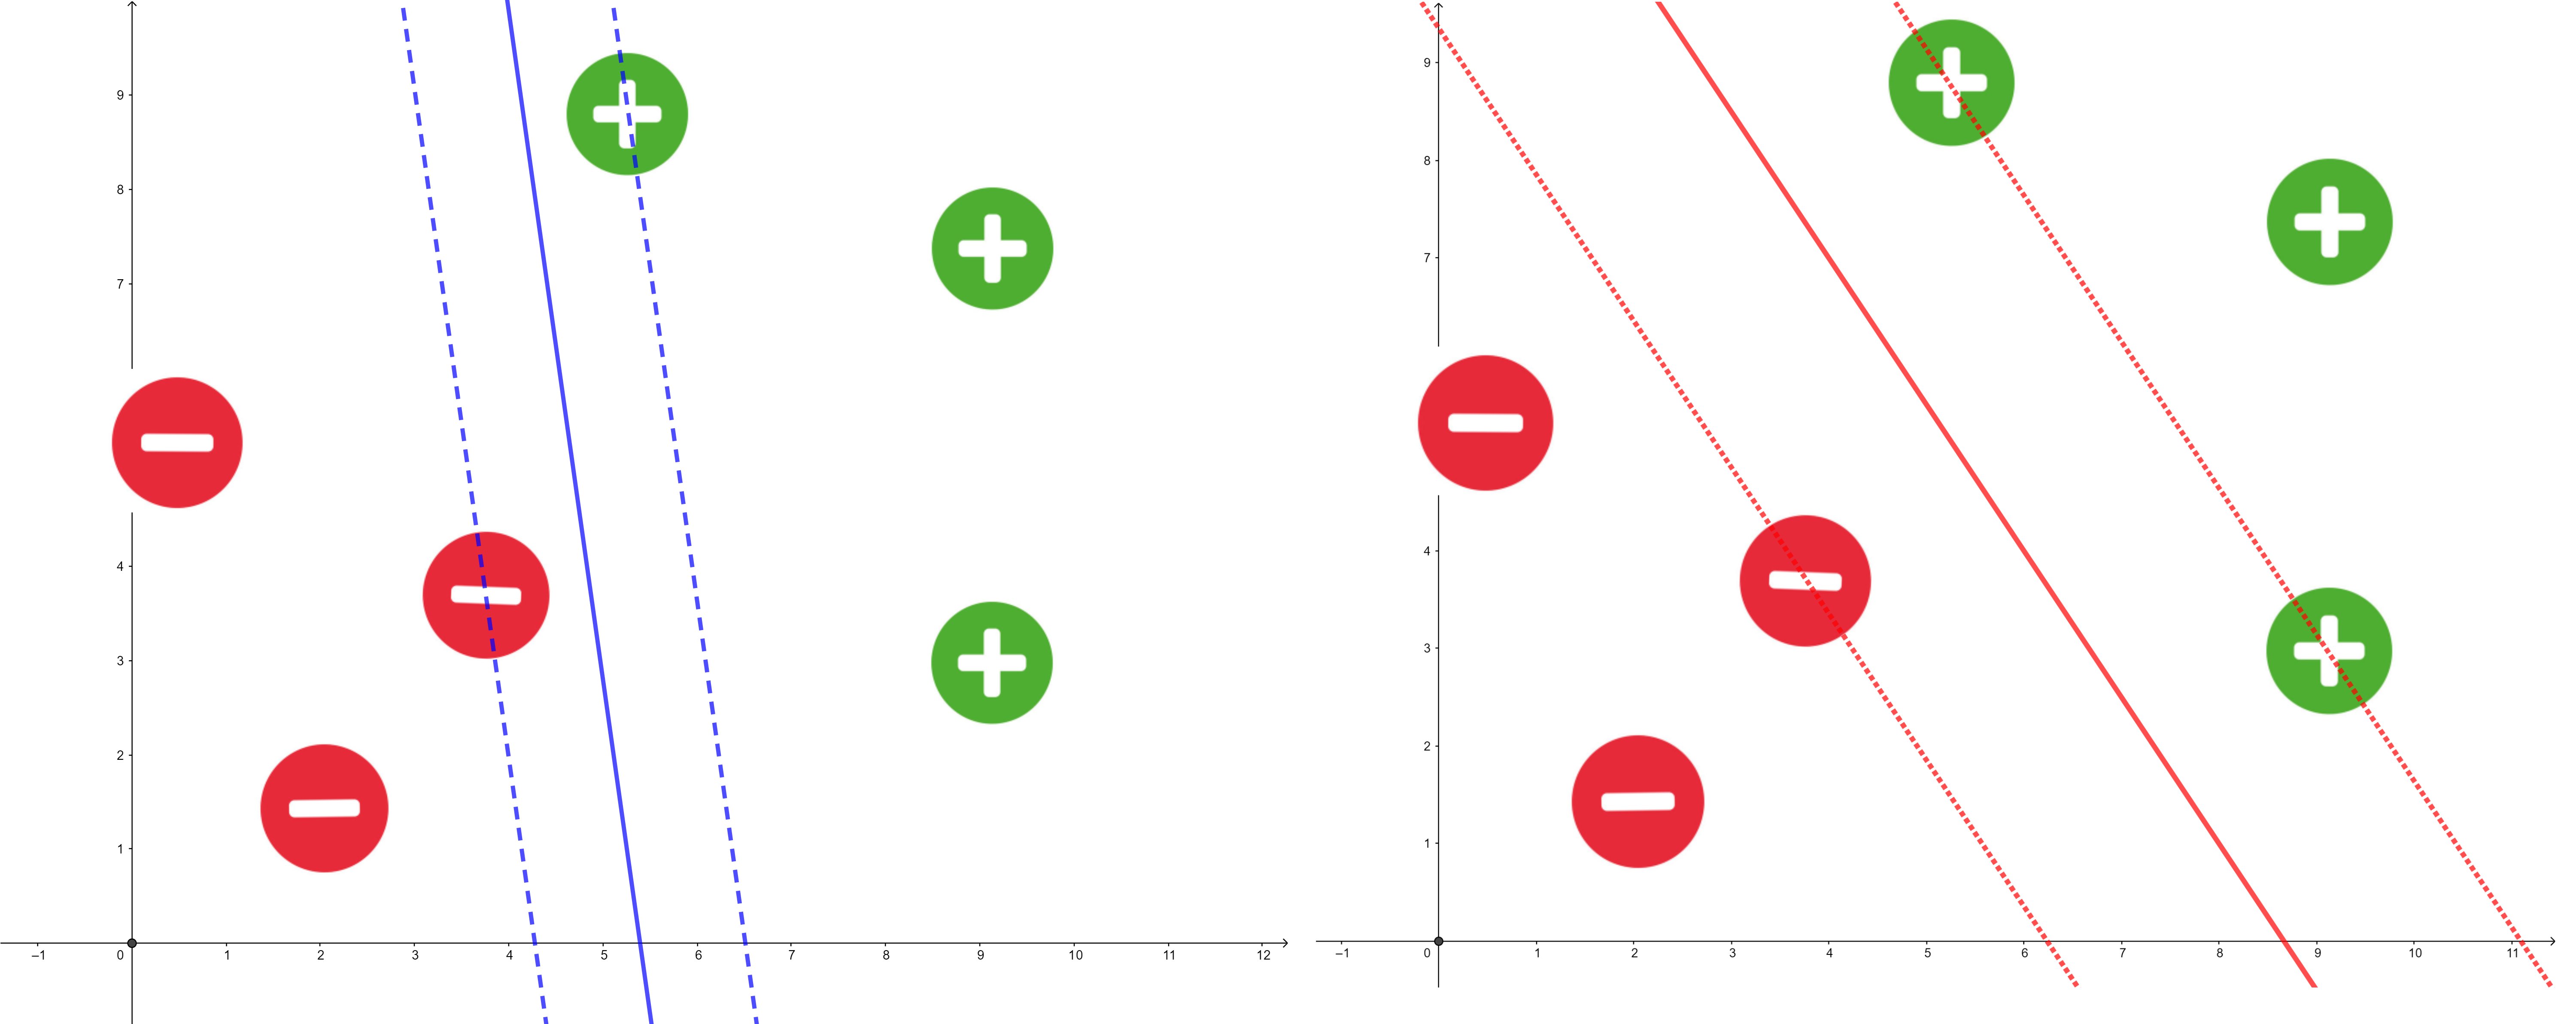
\includegraphics[width = 16cm]{assets/small_vs_big_margin.png}
	\caption{Abhängig von der Lage der Trennebene entstehen schmale (blau) oder breite (rot) Trennbänder. Das Ziel der \ac{SVM} ist die Maximierung der Breite des Trennbands durch die Ermittlung der optimalen Lage der Trennebene.}
	\label{fig:intuition_margin}
\end{figure}


\chapter{Hard-Margin Support Vector Machine} \label{sec:hard_margin}
Wie bereits in der Einführung erwähnt ist das Ziel einer Hard-Margin \ac{SVM} ist die Trennung zweier Klassen ohne Fehler mit einem möglichst breiten Trennband. Diese Aussage wird in diesem Kapitel mathematisch formuliert und als Optimierungsproblem dargestellt. Weiters wird beschrieben wie dieses Problem in die Standardform von \ac{QP} Problemen transformiert werden kann was für die Lösung nötig ist. 

\section{Problemdefinition} \label{sec:problem_def}
Gegeben sei ein Gewichtsvektor $w \in \mathbb{R}^{K}$, ein Bias $b \in \mathbb{R}$, ein beliebiger Punkt $x_{n} \in \mathbb{R}^{K}$ und ein zugehöriges Label $y_{n} \in \{-1, +1\}$. Eine Ebene im Raum kann allgemein definiert werden durch:

\begin{equation} \label{plane_eq}
    \begin{aligned}
    w^{T} x_{n} + b &= 0 \\
    \end{aligned}
\end{equation}

Mit einer bereits trainierten \ac{SVM} können neue, noch unklassifizierte Eingabevektoren $x_{n}$ wie folgt klassifiziert werden:

\begin{subequations} \label{svm_classify1}
	\begin{alignat}{2}
		y = sign(w^{T} x_{n} + b)  & \qquad & \text{ gleichbedeutend mit} \\
		w^{T} x_{n} + b > 0 & & \text{ für } y_{n} = +1\\
		w^{T} x_{n} + b < 0 & & \text{ für } y_{n} = -1
	\end{alignat}
\end{subequations}


Für die Herleitung führen wir eine noch striktere Regel ein. So soll für eine richtige Klassifikation eines gegebenen Eingabevektors $x_{n}$ mit dem Label $y_{n}$ gelten:
\begin{subequations} \label{decision_rules}
	\begin{alignat}{2}
		w^{T} x_{n} + b \geq +1 & \qquad & \text{ für } y_{n} = +1\\
		w^{T} x_{n} + b \leq -1 & & \text{ für } y_{n} = -1
	\end{alignat}
\end{subequations}


Durch \autoref{decision_rules} wird sichergestellt, dass Werte aus dem Intervall $\interval[open]{-1}{+1}$ als Ergebnis nicht vorkommen können. Wie in \autoref{fig:trennband} dargestellt entsteht dadurch ein symmetrisches Trennband um die Trennebene in dem keine Punkte liegen. Ziel der \ac{SVM} ist die Maximierung der Breite dieses Bandes.\\

\begin{figure}[H]
	\centering
	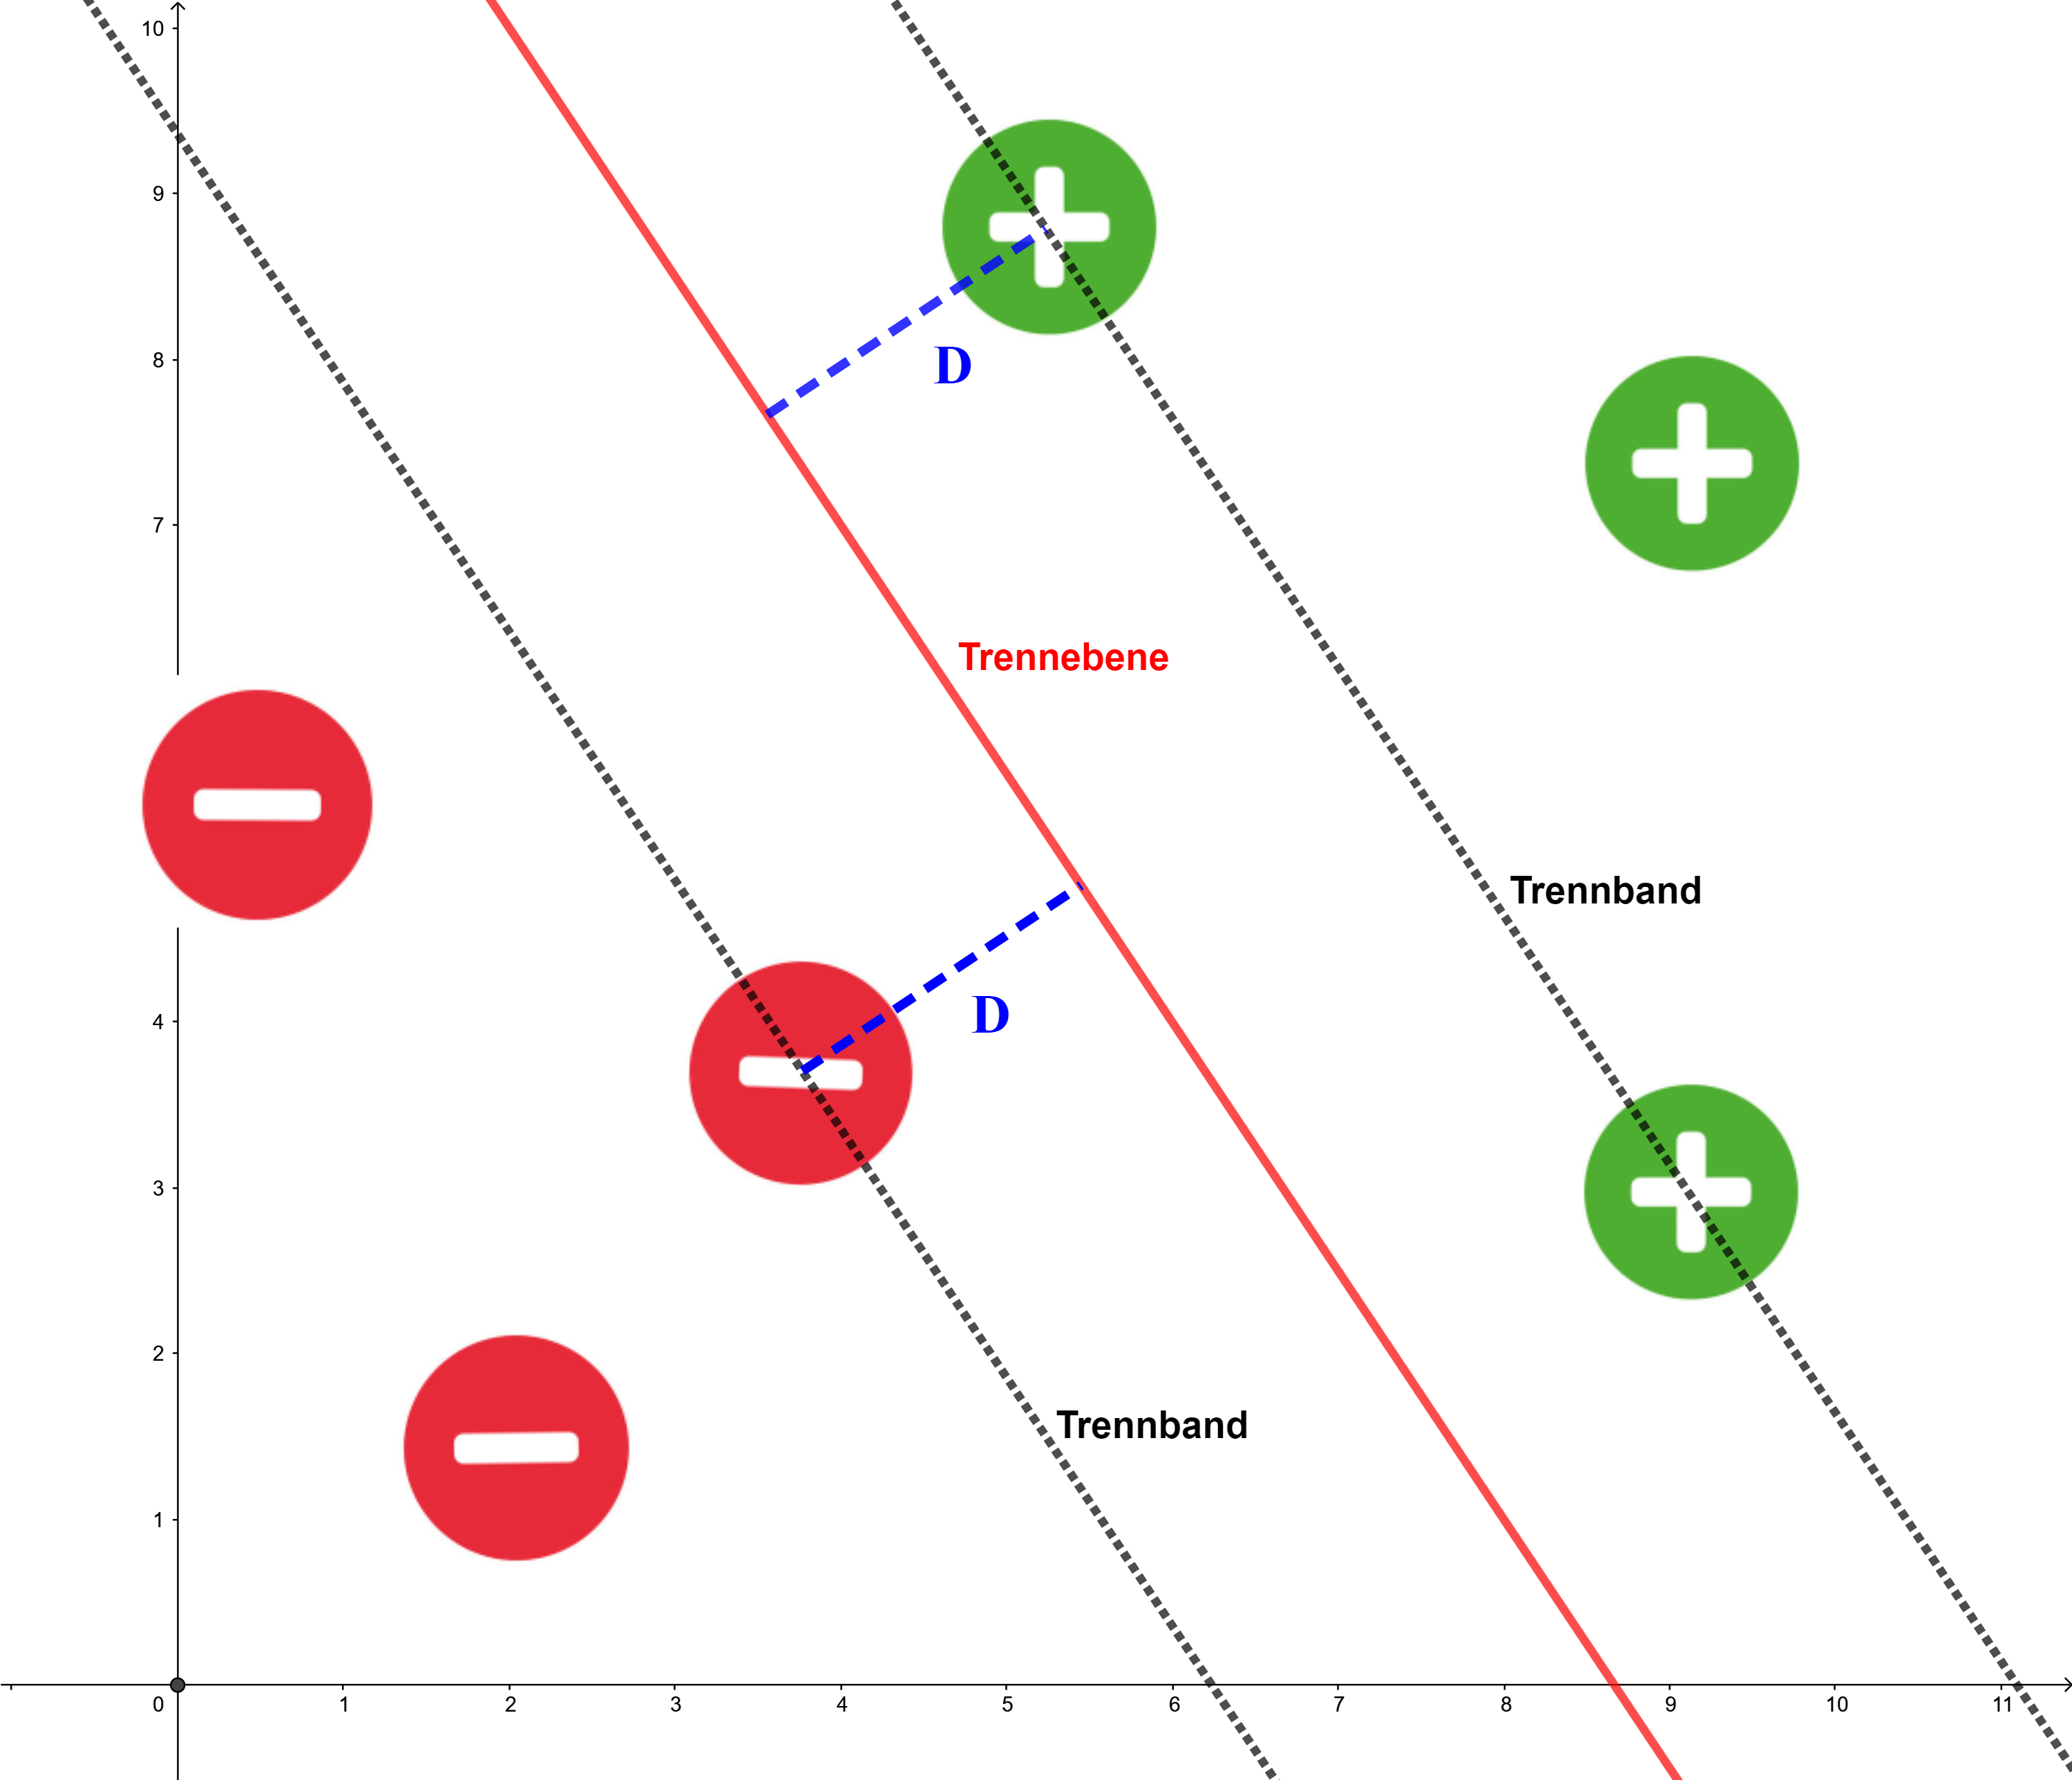
\includegraphics[width = 12cm]{assets/trennband.png}
	\caption{Um die Trennebene entsteht ein Trennband. Die am nächsten zu der Ebene liegenden Eingabevektoren liegen genau auf den Grenzen des Trennbands.}
	\label{fig:trennband}
\end{figure}



 \autoref{decision_rules} kann weiter verallgemeinert werden durch beidseitige Multiplikation mit $y_{n}$:

\begin{subequations} \label{decision_rules2}
	\begin{alignat}{2}
		y_{n} (w^{T} x_{n} + b) \geq 1 & \qquad & \text{ für } y_{n} = +1\\
		y_{n} (w^{T} x_{n} + b) \geq 1 & & \text{ für } y_{n} = -1
	\end{alignat}
\end{subequations}



Für den Fall, dass $x_{n} = \hat{x}$ genau an der Grenze des Trennbands liegt, gilt somit:
\begin{equation} \label{dec_rule}
	\begin{aligned}
		y_{n} (w^{T} \hat{x} + b) &= 1
	\end{aligned}
\end{equation}


Als nächsten Schritt bestimmen wir den euklidischen Normalabstand $D$ eines beliebigen Punkts $x_{n} \in \mathbb{R}^{K}$ zu der Ebene. Hierfür ist zuerst zu bemerken, dass $w$ normal zur definierten Ebene steht.

\begin{lemma}
	Eine Ebene sei definiert durch $w^{T} x + b = 0$. Der Vektor $w$ steht normal zu der definierten Ebene.
\end{lemma}

\begin{proof}
	Man wähle zwei Punkte $x_{1}, x_{2} \in \mathbb{R}^{K}$ die auf der Ebene liegen. Somit muss gelten:
	\begin{equation}
		\begin{aligned}
			w^{T} x_{1} + b &= 0 \\
			w^{T} x_{2} + b &= 0 \\
			w^{T} (x_{1} - x_{2}) &= 0 \leftrightarrow \norm{w^{T}} \norm{x_{1} - x_{2}} \cos(\alpha) = 0 \leftrightarrow \alpha = 90^{\circ}
		\end{aligned}
	\end{equation}
\end{proof}

Um den Normalabstand $d$ eines beliebigen Punkts $x_{n}$ zu ermitteln wählt man einen Punkt $x$, der auf der Ebene liegt, und projiziert den Vektor $(x_{n} - x)$ auf den Einheitsvektor von $w$. Weil nur der tatsächliche Abstand zur Ebene relevant ist und nicht die Richtung nimmt man den Betrag.

\begin{equation} \label{distance_to_plane}
	\begin{aligned}
		d &= | \frac{w^{T}}{\lVert w \rVert} (x_{n} - x) | = \\
		&= \frac{1}{\norm{w}} | (w^{T} x_{n} - w^{T} x) | =\\
		&= \frac{1}{\norm{w}} | (w^{T} x_{n} + b - (w^{T} x + b)) |
	\end{aligned}
\end{equation}

\begin{figure}[H]
	\centering
	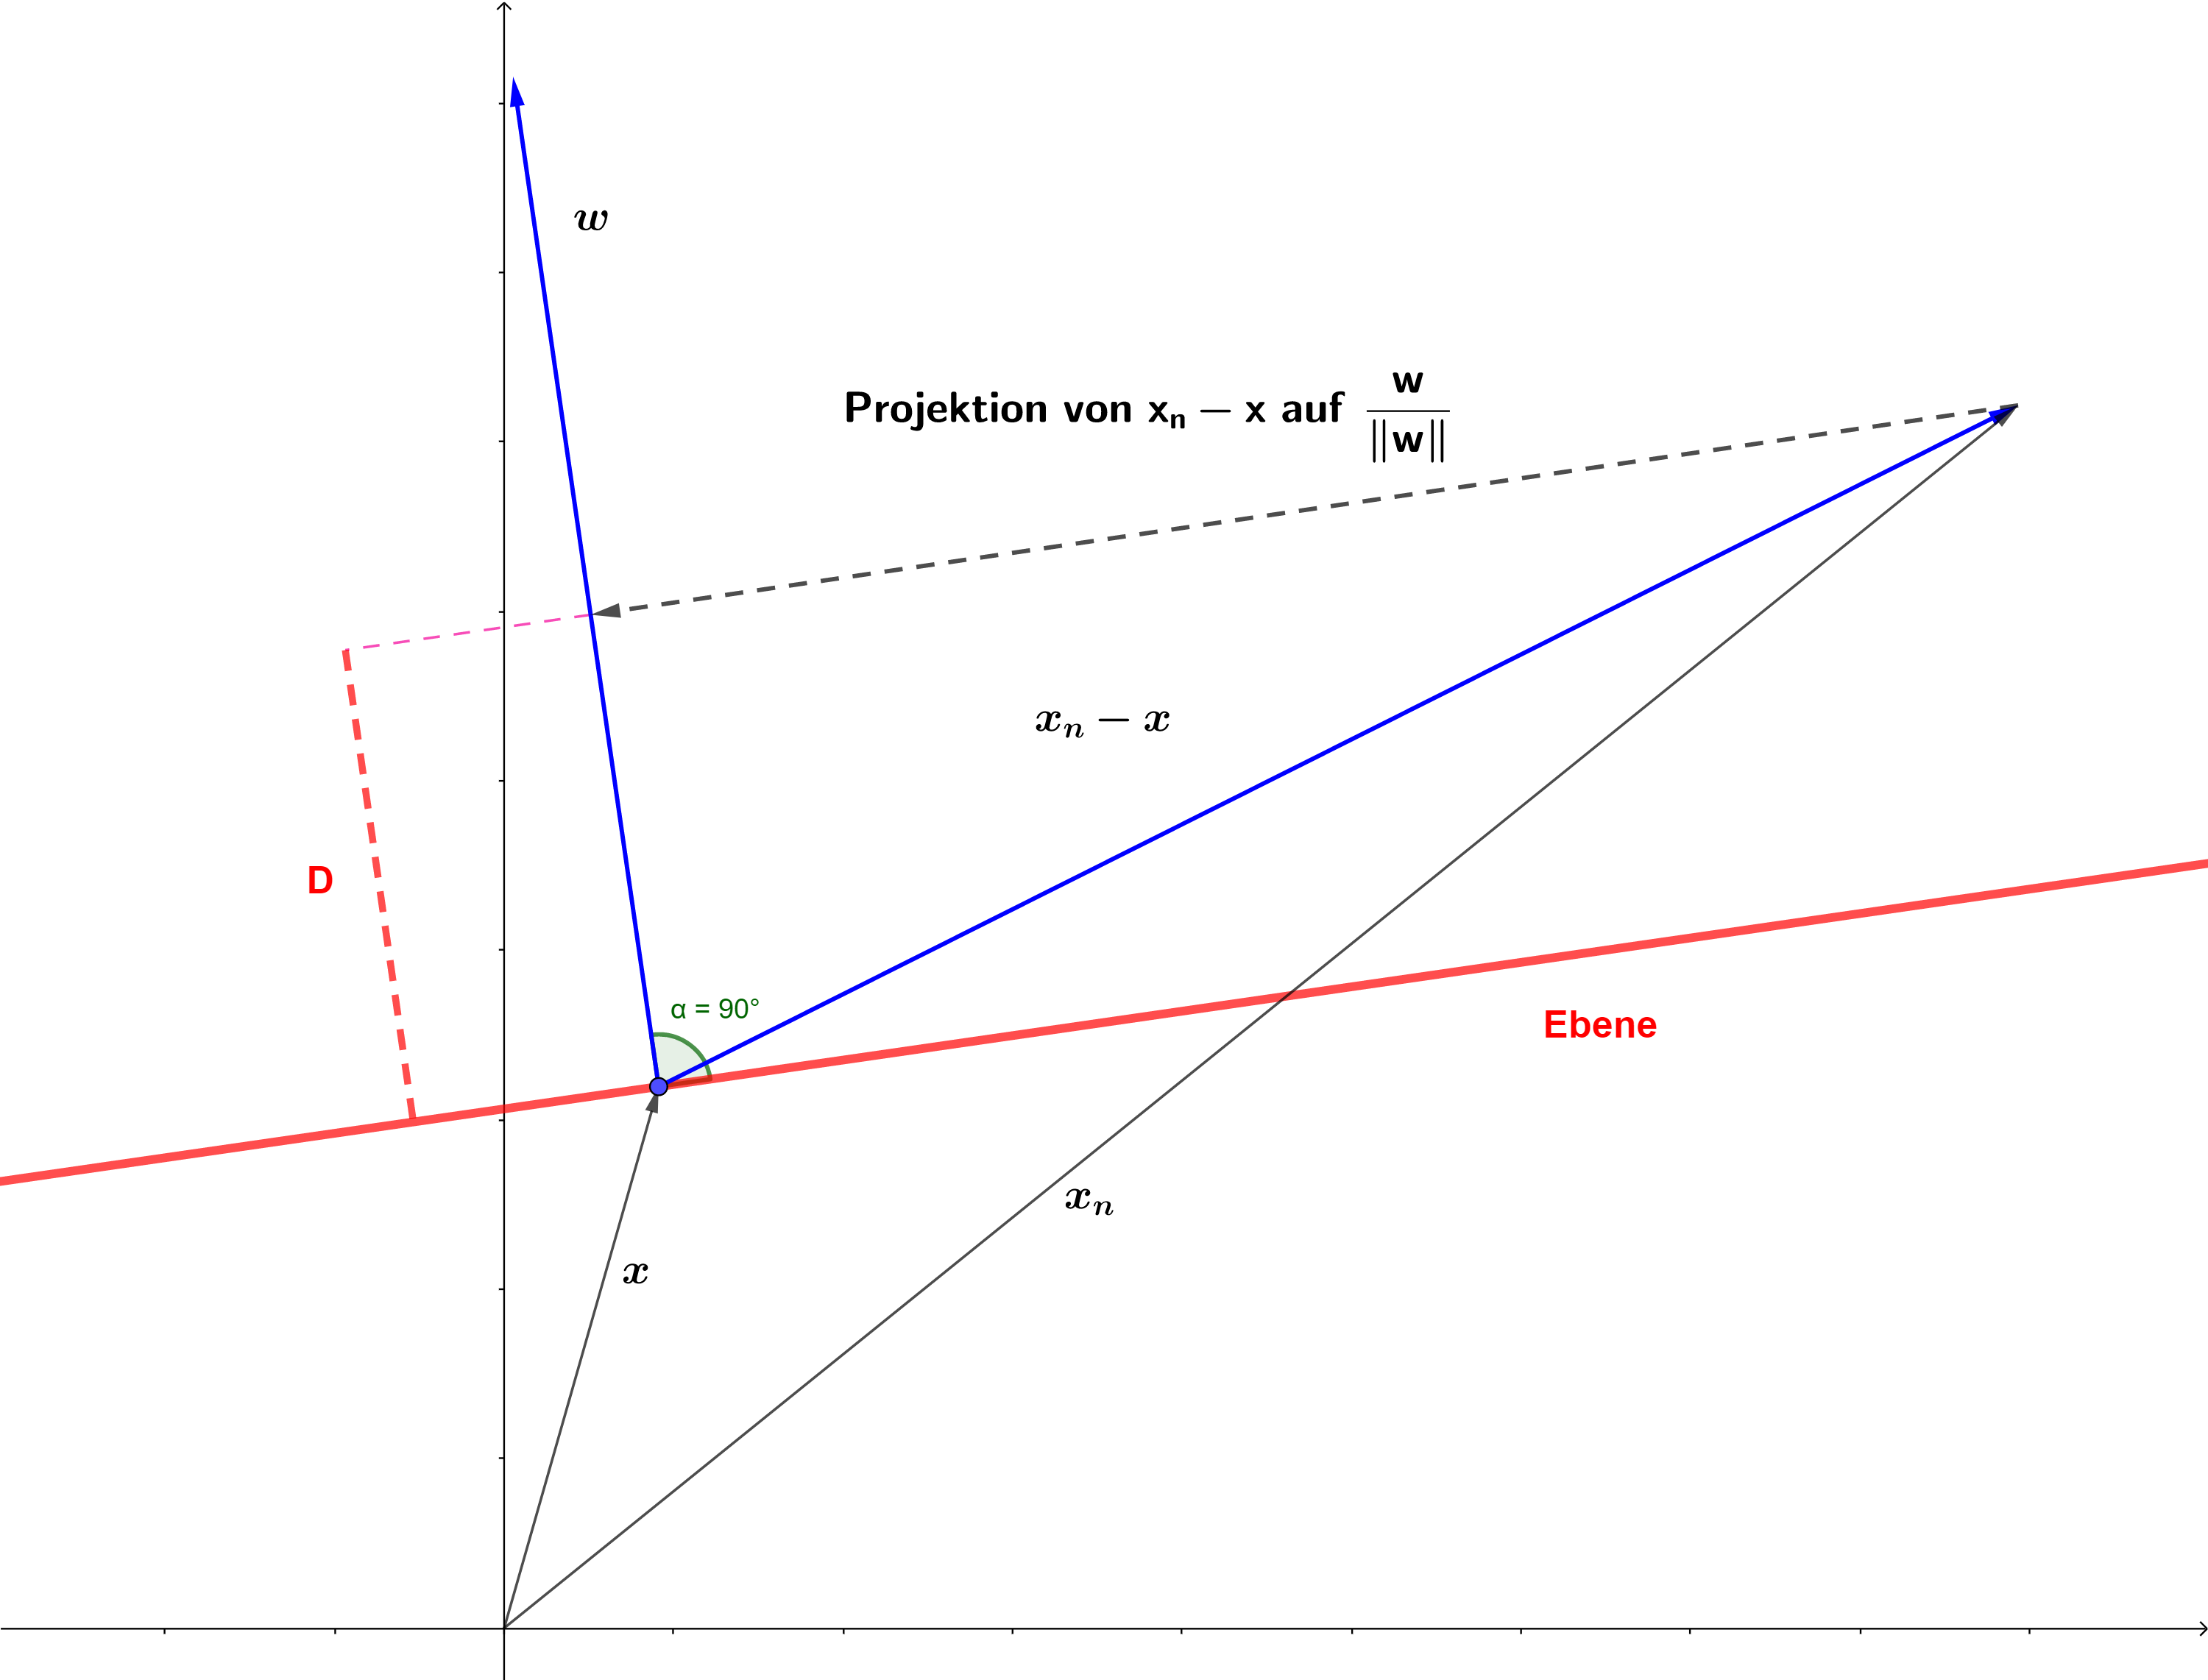
\includegraphics[width = 13cm]{assets/projection.png}
	\caption{Durch die Projektion von $(x_{n} - x)$ auf den Einheitsvektor von $w$ kann der Normalabstand $d$ von $x_{n}$ zu der Ebene bestimmt werden.}
	\label{fig:projection}
\end{figure}

Weil der Punkt $x$ auf der Ebene liegt gilt $w^{T} x + b = 0$ (\autoref{plane_eq}):
\begin{equation} \label{distance_to_plane_simplified1}
	\begin{aligned}
		d &= \frac{1}{\norm{w}} | (w^{T} x_{n} + b) |
	\end{aligned}
\end{equation}

Trifft man nun die Annahme, dass $x_{n} = \hat{x}$ der am nächsten zu der Trenngrenze liegende Punkt ist, so gilt aus \autoref{dec_rule} $y_{k} (w^{T} \hat{x} + b) = 1 = |w^{T} \hat{x} + b|$ unter der Annahme, dass der Punkt richtig klassifiziert wurde. Somit ergibt sich der kleinste Abstand zur Trennebene $D = d(\hat{x})$, welcher zugleich der halben Breite des Trennbands entspricht, als:
\begin{equation} \label{distance_to_plane_simplified2}
	\begin{aligned}
		D &= \frac{1}{\norm{w}}
	\end{aligned}
\end{equation}

\begin{figure}[H]
	\centering
	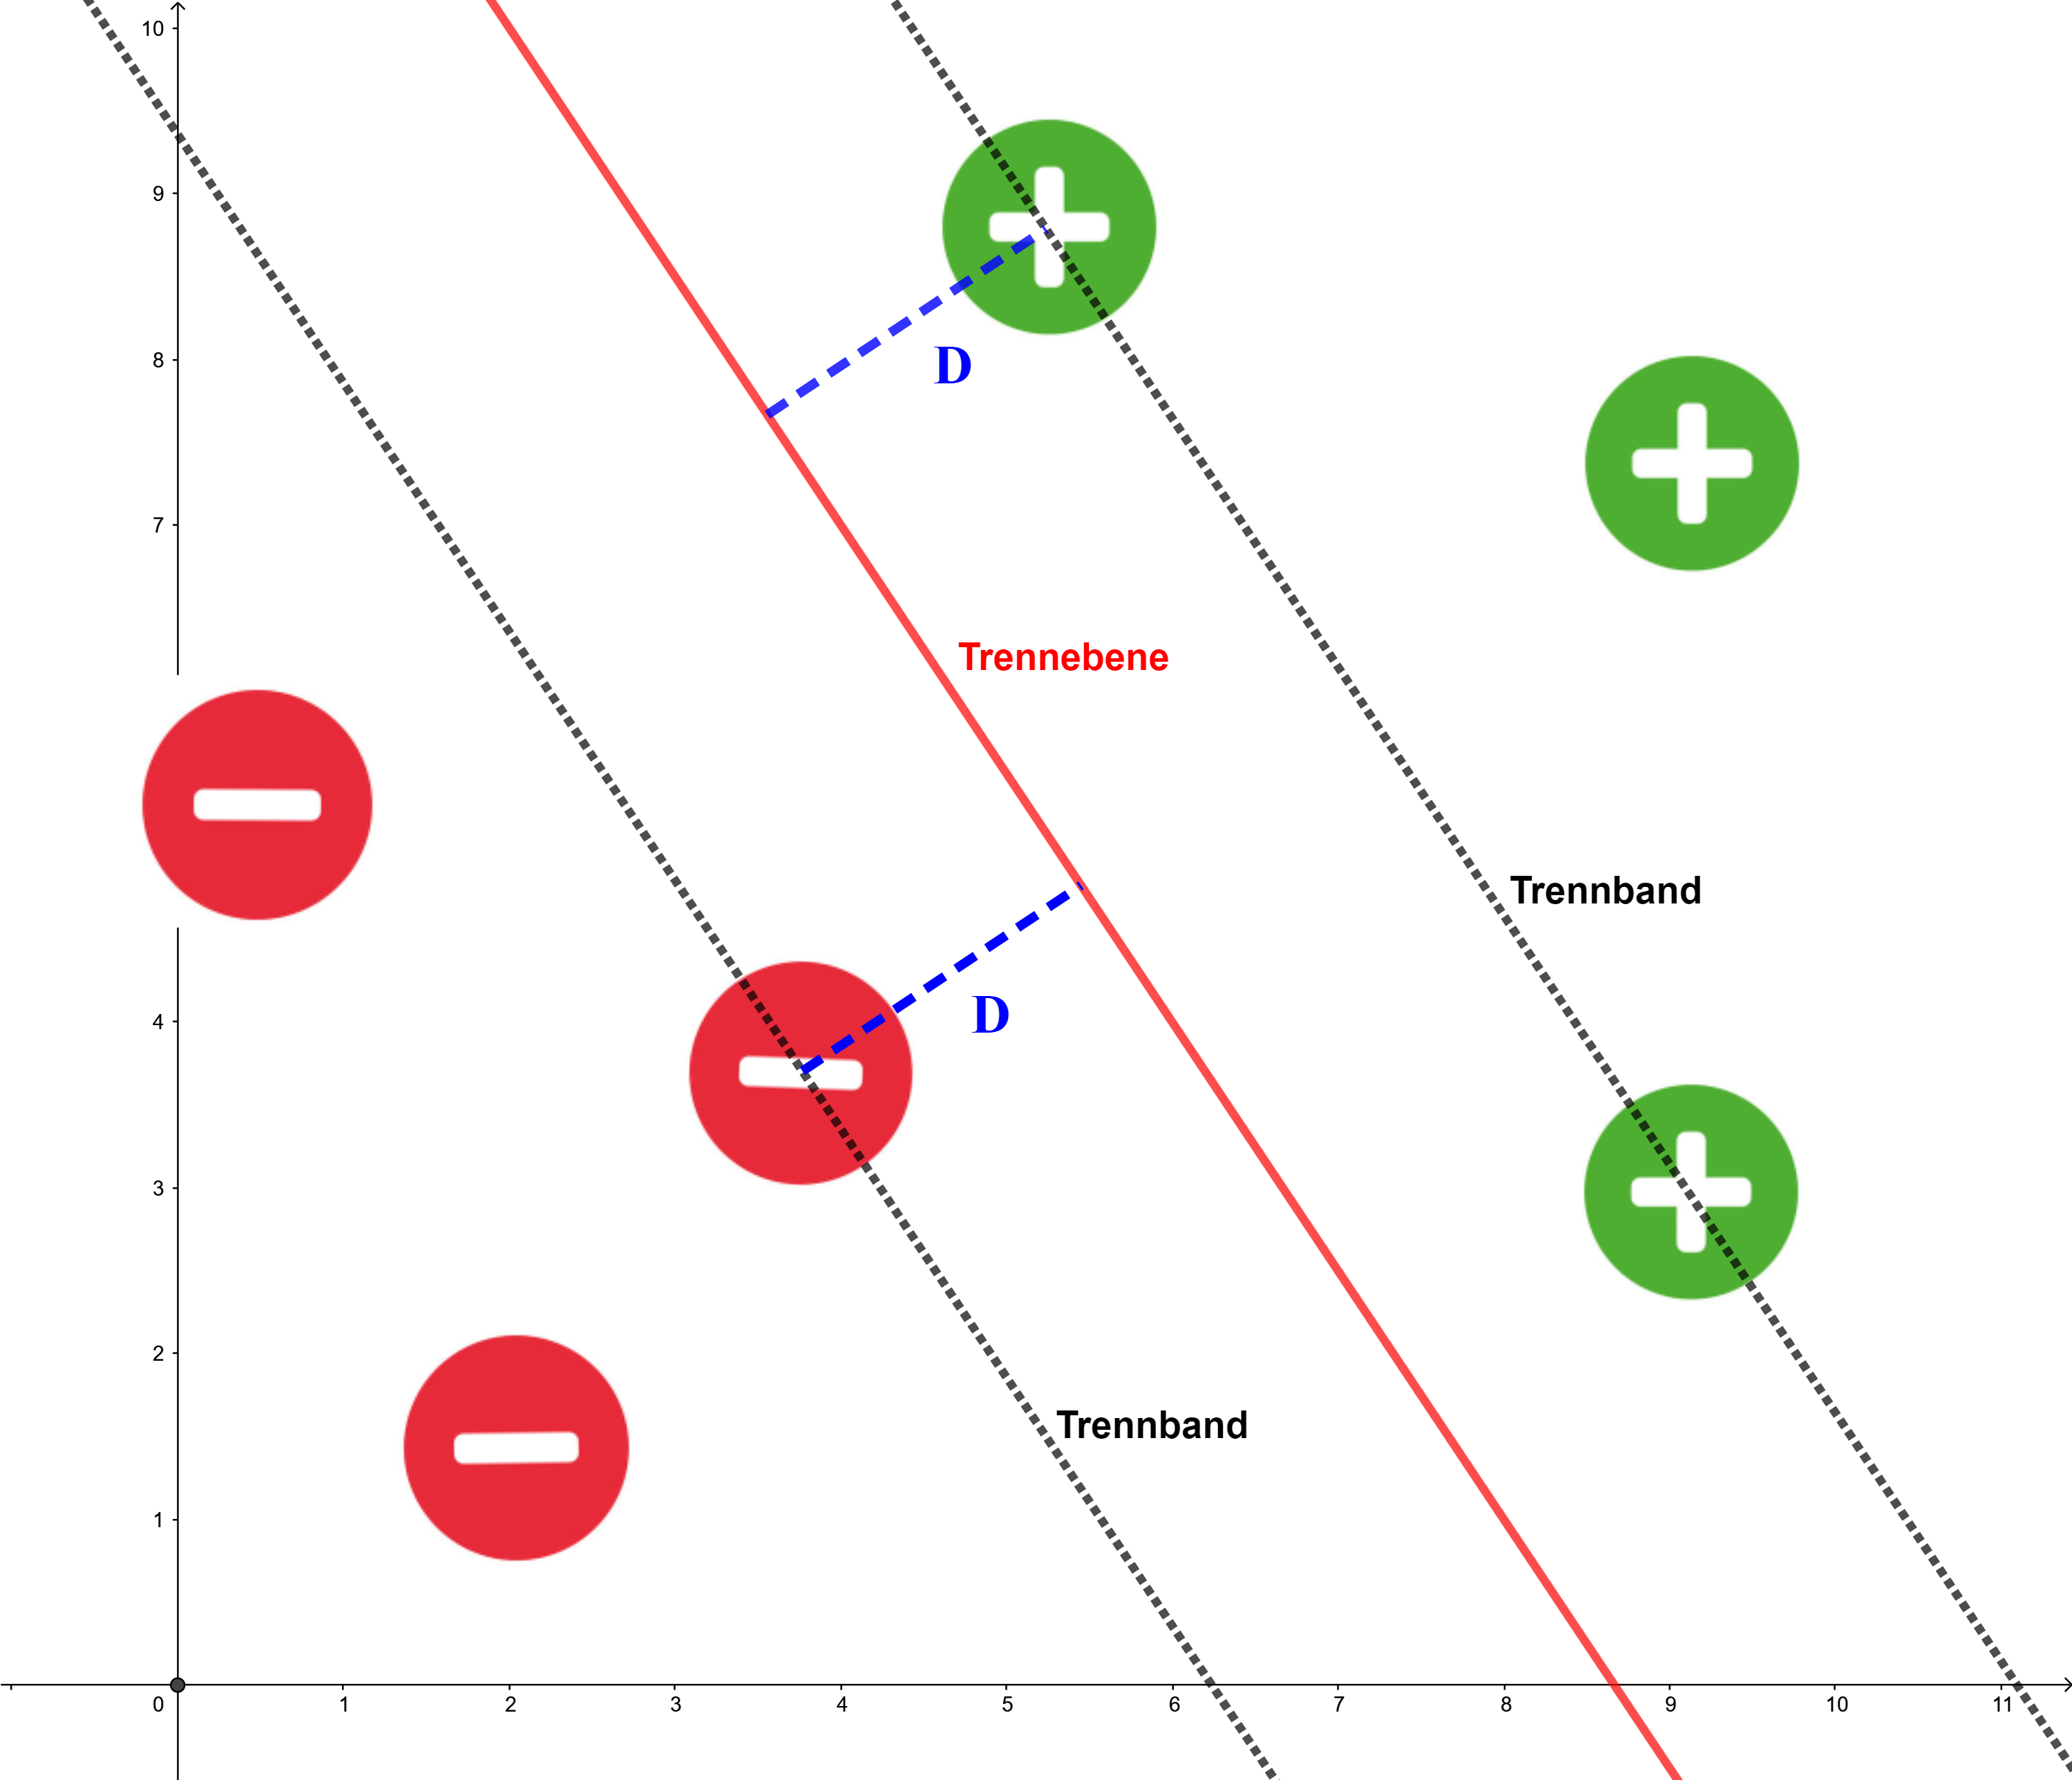
\includegraphics[width = 12cm]{assets/trennband_mit_D.png}
	\caption{Der Normalabstand $D$ von der Ebene zu den am nächsten liegenden Eingabevektoren entspricht genau der Hälfte der Breite des Trennbands.}
	\label{fig:trennband2}
\end{figure}


\section{Optimierungsproblem}

\autoref{distance_to_plane_simplified2} beschreibt den Normalabstand zu dem am nächsten an der Ebene liegenden Punkt $\hat{x}$. Der Normalabstand ist gleichbedeutend mit der Hälfte der Breite des Trennbands, wobei für die Optimierung der Faktor $2$ keine Rolle spielt und vernachlässigt werden kann. \\
Das Ziel einer \ac{SVM} ist die Maximierung der Breite des Trennbands für $N$ Eingabevektoren $\{x_{1}..x_{N}\}, x_{n} \in \mathbb{R}^{K}$. 

Bei dem beschriebenen Problem handelt es sich um ein Optimierungsproblem mit Nebenbedingungen:

\begin{subequations}
	\begin{alignat}{2}
		&\!\max_{w}        &\qquad&  \frac{1}{\norm{w}} \label{eq:optProb}\\
		&\text{mit } &      & \min_{n=1..N} |w^{T} x_{n} + b| = 1 \label{eq:constraint1}
	\end{alignat}
\end{subequations}

\autoref{eq:constraint1} beschreibt hier den am nächsten zur Ebene gelegenen Punkt $\hat{x}$ aus der gebenenen Menge von Eingabevektoren in allgemeiner Form. Der Betrag lässt sich vermeiden durch die Anwendung von \autoref{decision_rules2}:

\begin{equation} \label{abs_value_trick}
	\begin{aligned}
		|w^{T} x_{n} + b| &= y_{n} (w^{T} x_{n} + b)
	\end{aligned}
\end{equation}


Durch Anwendung von \autoref{abs_value_trick} in \autoref{eq:constraint1}, Umformulierung der Maximierung in eine Minimierung und der Verallgemeinerung von $\hat{x}$ auf beliebige Punkte $x_{n}$ erhält man:
\begin{subequations}
	\begin{alignat}{2}
		&\!\min_{w}        &\qquad&  \frac{1}{2} w^{T} w \label{eq:optProb2}\\
		&\text{mit } &      & y_n (w^{T} x_{n} + b) \geq 1 \text{ für } n=1..N \label{eq:constraint12}
	\end{alignat}
\end{subequations}

Die Verallgemeinerung von \autoref{eq:constraint1} auf \autoref{eq:constraint12} auf beliebige Punkte ist so möglich, weil durch \autoref{dec_rule} sichergestellt ist, dass für beliebige Punkte $y_{n}(w^{T} x_{n} + b) \geq 1$ gilt.



\section{Lagrange Optimierung} \label{sec:lagrange}

Das beschriebene Optimierungsproblem beinhaltet eine Ungleichung in \autoref{eq:constraint12}. Um die Lagrangegleichung aufstellen zu können wird zuerst die Nebenbedingung umgeformt:
\begin{subequations} \label{min_problem}
	\begin{alignat}{2}
		&\!\min_{w}        &\qquad&  \frac{1}{2} w^{T} w \label{eq:optProb3}\\
		&\text{mit } &      & y_n (w^{T} x_{n} + b)-1 \geq 0 \text{ für } n=1..N \label{eq:constraint13}
	\end{alignat}
\end{subequations}

Das Problem kann nun als Lagrangegleichung dargestellt werden:
\begin{subequations}
	\begin{alignat}{2}
		&\!\min_{w, b}        &\qquad&  \Lagr (w, b, \alpha) = \frac{1}{2} w^{T} w - \sum_{n=1}^{N} \alpha_{n} (y_n (w^{T} x_{n} + b)-1) \label{eq:optProb4}\\
		&\max_{\alpha_{n}} &      & \alpha_{n} \geq 0 \text{ für } n=1..N \label{eq:constraint14}
	\end{alignat}
\end{subequations}
 Weil \autoref{eq:constraint13} eine Ungleichung der Form $\geq 0$ beinhaltet werden diese Terme von der zu maximierenden Funktion subtrahiert. Nun kann die uneingeschränkte Optimierung von \autoref{eq:optProb4} nach $w$ und $b$ durchgeführt werden indem die Ableitungen bestimmt und $0$ gesetzt werden:

\begin{equation} \label{gradient_lagrange_w}
	\begin{aligned}
		\nabla_{w} \Lagr &= w - \sum_{n=1}^{N} \alpha_{n} y_{n} x_{n} \overset{!}{=} \vec{0} \\
		w &= \sum_{n=1}^{N} \alpha_{n} y_{n} x_{n}
	\end{aligned}
\end{equation}

\begin{equation} \label{partial_lagrange_b}
	\begin{aligned}
		\frac{\partial}{\partial b} \Lagr &= - \sum_{n=1}^{N} \alpha_{n} y_{n} \overset{!}{=} 0 \\
		\sum_{n=1}^{N} \alpha_{n} y_{n} &= 0
	\end{aligned}
\end{equation}

Die Ergebnisse von \autoref{gradient_lagrange_w} und \autoref{partial_lagrange_b} können in \autoref{eq:optProb4} eingesetzt werden. Hierfür wird zuerst die Summe in \autoref{eq:optProb4} in Teilsummen zerlegt:

\begin{equation} \label{lagrange_substituted}
	\begin{aligned}
		\Lagr(w, b, \alpha) &= \frac{1}{2} w^{T} w - \sum_{n=1}^{N} \alpha_{n} (y_n (w^{T} x_{n} + b)-1) = \\
		&= \frac{1}{2} w^{T} w - [\sum_{n=1}^{N} \alpha_{n} y_{n} b - \sum_{n=1}^{N} \alpha_{n} + \sum_{n=1}^{N} \alpha_{n} y_{n} w^{T} x_{n}]
	\end{aligned}
\end{equation}

Weil $\sum_{n=1}^{N} \alpha_{n} y_{n} = 0$ (\autoref{partial_lagrange_b}) gilt fällt der Term $\sum_{n=1}^{N} \alpha_{n} y_{n} b$ weg:
\begin{equation} \label{lagrange_substituted2}
	\begin{aligned}
		\Lagr(w, b, \alpha) &= \frac{1}{2} w^{T} w - [-\sum_{n=1}^{N} \alpha_{n} + \sum_{n=1}^{N} \alpha_{n} y_{n} w^{T} x_{n}]
	\end{aligned}
\end{equation}

Vergleicht man den Term $\sum_{n=1}^{N} \alpha_{n} y_{n} w^{T} x_{n}$ mit dem Ergebnis von \autoref{gradient_lagrange_w} erkennt man, dass $\sum_{n=1}^{N} \alpha_{n} y_{n} w^{T} x_{n} = w^T w$ gilt. Dies kann ausgeschrieben werden als:
\begin{equation} \label{lagrange_substituted3}
	\begin{aligned}
		\Lagr(\alpha) &= \sum_{n=1}^{N }\alpha_{n} - \frac{1}{2} \sum_{n=1}^{N} \sum_{m=1}^{M} y_{n} y_{m} \alpha_{n} \alpha_{m} x_{n}^{T} x_{m}
	\end{aligned}
\end{equation}

\autoref{lagrange_substituted3} beschreibt das Optimierungsproblem ohne Abhängigkeit von $w$ und $b$, wir haben jetzt also eine Maximierung für $\alpha$ mit Nebenbedingungen:
\begin{subequations} \label{final_lagrange}
	\begin{alignat}{2}
		&\!\max_{\alpha}        &\qquad&  	\Lagr(\alpha) = \sum_{n=1}^{N} \alpha_{n} - \frac{1}{2} \sum_{n=1}^{N} \sum_{m=1}^{M} y_{n} y_{m} \alpha_{n} \alpha_{m} x_{n}^{T} x_{m} \label{eq:optProb5}\\
		&\text{mit } &      & \alpha_{n} \geq 0 \text{ für } n=1..N \label{eq:constraint16}\\
		&       & & \sum_{n=1}^{N} \alpha_{n} y_{n} = 0\text{ für } n=1..N \label{eq:constraint17}
	\end{alignat}
\end{subequations}

Bei dem in \autoref{final_lagrange} beschriebene Problem handelt es sich um ein Quadratic Programming Problem, ersichtlich an dem Term $x_{n}^{T} x_{m}$, welches beispielsweise mittels eines Quadratic Programming Solvers gelöst werden kann. Als Ergebnis erhält man einen Vektor $\alpha$ mit allen $\alpha_{n}$. Durch Einsetzen in $w = \sum_{n=1}^{N} \alpha_{n} y_{n} x_{n}$ kann $w$ bestimmt werden. \\

Betrachtet man den Ergebnisvektor $\alpha$ so wird man feststellen, dass sehr viele Werte $0$ ergeben. In \autoref{eq:optProb4} befindet sich der Term $\alpha_{n} (y_n (w^{T} x_{n} + b)-1)$. Der Term $(y_n (w^{T} x_{n} + b)-1)$ kann als Schlupf bezeichnet werden. Das Produkt von Schlupf und $\alpha_{n}$ kann nur $0$ werden wenn entweder der Schlupf $0$ ist oder $\alpha_{n}$. Umgekehrt bedeutet dies, dass alle Vektoren, die einen minimalen Abstand zu der Trennebene haben, ein $\alpha_{n} \neq 0$ aufweisen. Vektoren, die diese Bedingung erfüllen, werden Stützvektoren genannt. \\


Mit dieser Erkenntnis kann \autoref{gradient_lagrange_w} erneut analysiert werden:

\begin{equation} \label{weights_calc}
	\begin{aligned}
		w &= \sum_{n=1}^{N} \alpha_{n} y_{n} x_{n}
	\end{aligned}
\end{equation}

Weil nur Stützvektoren ein $\alpha_{n} \neq 0$ aufweisen und somit auch nur Stützvektoren einen Beitrag zu $w$ leisten, kann \autoref{weights_calc} stark vereinfacht werden:

\begin{equation} \label{weights_calc2}
	\begin{aligned}
		w &= \sum_{n \text{ ist Stützvektor}} \alpha_{n} y_{n} x_{n}
	\end{aligned}
\end{equation}

Der Gewichtsvektor $w$ hängt also lediglich von den Stützvektoren ab, deren Anzahl in der Regel gering ist.\\


Noch offen ist die Bestimmung des Bias $b$. Weil für Stützvektoren $y_n (w^{T} x_{n} + b) = 1$ gilt (\autoref{dec_rule}) kann der Bias $b$ aus jedem beliebigen Stützvektor bestimmt werden:

\begin{equation} \label{bias_calc}
	\begin{aligned}
		b &= \frac{1}{y_{n}} - w^{T} x_{n} = \\
		&= y_{n} - w^{T} x_{n}
	\end{aligned}
\end{equation}



\section{Lösung mittels Quadratic Programming Solver} \label{sec:qp}

Weil es sich bei dem in \autoref{final_lagrange} beschriebene Optimierungsproblem um ein Quadratic Programming Problem handelt kann dieses auch mittels eines Quadratic Programming Solvers gelöst werden. Die Implementationsdetails für diese Lösungsverfahren werden an dieser Stelle nicht weiter ausgeführt. Für die Anwendung eines Quadratic Programming Solvers muss das Problem in die Standardform von \ac{QP} Problemen umformuliert werden:

\begin{equation} \label{std_QP_problem}
	\begin{aligned}
		\min_{x} &= \frac{1}{2} x^{T} Q x + c x + d 
	\end{aligned}
\end{equation}

$Q \in \mathbb{R}^{n \times n}$ ist eine symmetrische reelle Matrix mit Koeffizienten, die einen quadratischen Beitrag leisten. $c \in \mathbb{R}$ ist ein Faktor für den linearen Beitrag und $d \in \mathbb{R}$ ist ein fixer Anteil. \\

Unter der Voraussetzung, dass $\max_{x} f(x) = \min_{x} (-f(x))$ gilt können wir unser Maximierungsproblem aus \autoref{final_lagrange} in ein Minimierungsproblem umformen:
\begin{equation} \label{qp_adapt1}
	\begin{aligned}
		\min_{\alpha} \Lagr(\alpha) &= \frac{1}{2} \sum_{n=1}^{N} \sum_{m=1}^{M} y_{n} y_{m} \alpha_{n} \alpha_{m} x_{n}^{T} x_{m} - \sum_{n=1}^{N} \alpha_{n}
	\end{aligned}
\end{equation}

Als nächsten Schritt müssen wir die Koeffizienten aus den Summen extrahieren, $\alpha$ und $y$ als Vektor darstellen, das Problem in die Standard-QP-Form bringen und die Nebenbedingungen als Matrizenmultiplikation darstellen:


\begin{subequations} \label{qp1}
	\begin{alignat}{2}
		&\!\min_{\alpha}        &\qquad& \Lagr(\alpha) = \frac{1}{2} \alpha^{T} Q \alpha + (-1^T) \alpha \label{eq:qp1}\\
		&\text{mit} &      & Q = \begin{bmatrix} 
			y_{1}y_{1}x_{1}^{T}x_{1} & y_{1}y_{2}x_{1}^{T}x_{2} & \dots & y_{1}y_{N}x_{1}^{T}x_{N}\\
			y_{2}y_{1}x_{2}^{T}x_{1} & y_{2}y_{2}x_{2}^{T}x_{2} & \dots & y_{2}y_{N}x_{2}^{T}x_{N}\\
			\vdots & \vdots & \vdots & \vdots\\
			y_{N}y_{1}x_{N}^{T}x_{1} & y_{N}y_{2}x_{N}^{T}x_{2} & \dots & y_{N}y_{N}x_{N}^{T}x_{N}\\ 
	\end{bmatrix}\\
&\text{für} & & y^{T} \alpha = 0\\
& & & 0 \leq \alpha \leq \infty
	\end{alignat}
\end{subequations}

An dieser Stelle ist zu bemerken dass es sich bei der Matrix $Q$ um eine $N \times N$ Matrix handelt. Für eine große Anzahl an Trainingsdaten ist dies sehr problematisch beziehungsweise nicht mehr lösbar. Hier können andere Optimierungsverfahren wie beispielsweise in \textcite{platt_sequential_1998} beschrieben verwendet werden. \\


In dieser Darstellung kann das Problem direkt an ein Quadratic-Programming Solver Framework übergeben werden. Als Ergebnis erhalten wir einen Vektor $\alpha = (\alpha_{1}, \alpha_{2}, ..., \alpha_{n})$. \\

Daraus kann, wie bereits zuvor erwähnt, $w$ und $b$ bestimmt werden:

\begin{equation} \label{weights_calc_qp}
	\begin{aligned}
		w &= \sum_{n=1}^{N} \alpha_{n} y_{n} x_{n}
	\end{aligned}
\end{equation}

Für die Biasberechnung wird ein beliebiger Stützvektor $x_{k}$ benötigt. Dieser kann bestimmt werden indem der Ergebnisvektor $\alpha$ betrachtet wird. Ein Stützvektor $x_{k}$ muss $\alpha_{k} \neq 0$ aufweisen.
\begin{equation} \label{bias_calc_qp}
	\begin{aligned}
		b &= \frac{1}{y_{k}} - w^{T} x_{k}
	\end{aligned}
\end{equation}

Die \ac{SVM} ist nun vollständig definiert, neue Eingabevektoren $x$ können wie folgt klassifiziert werden:
\begin{equation} \label{svm_classify}
	\begin{aligned}
		y &= sign(w^{T} x + b)
	\end{aligned}
\end{equation}

\chapter{Soft-Margin Support Vector Machine} \label{sec:soft_margin}
\begin{figure}[H]
	\centering
	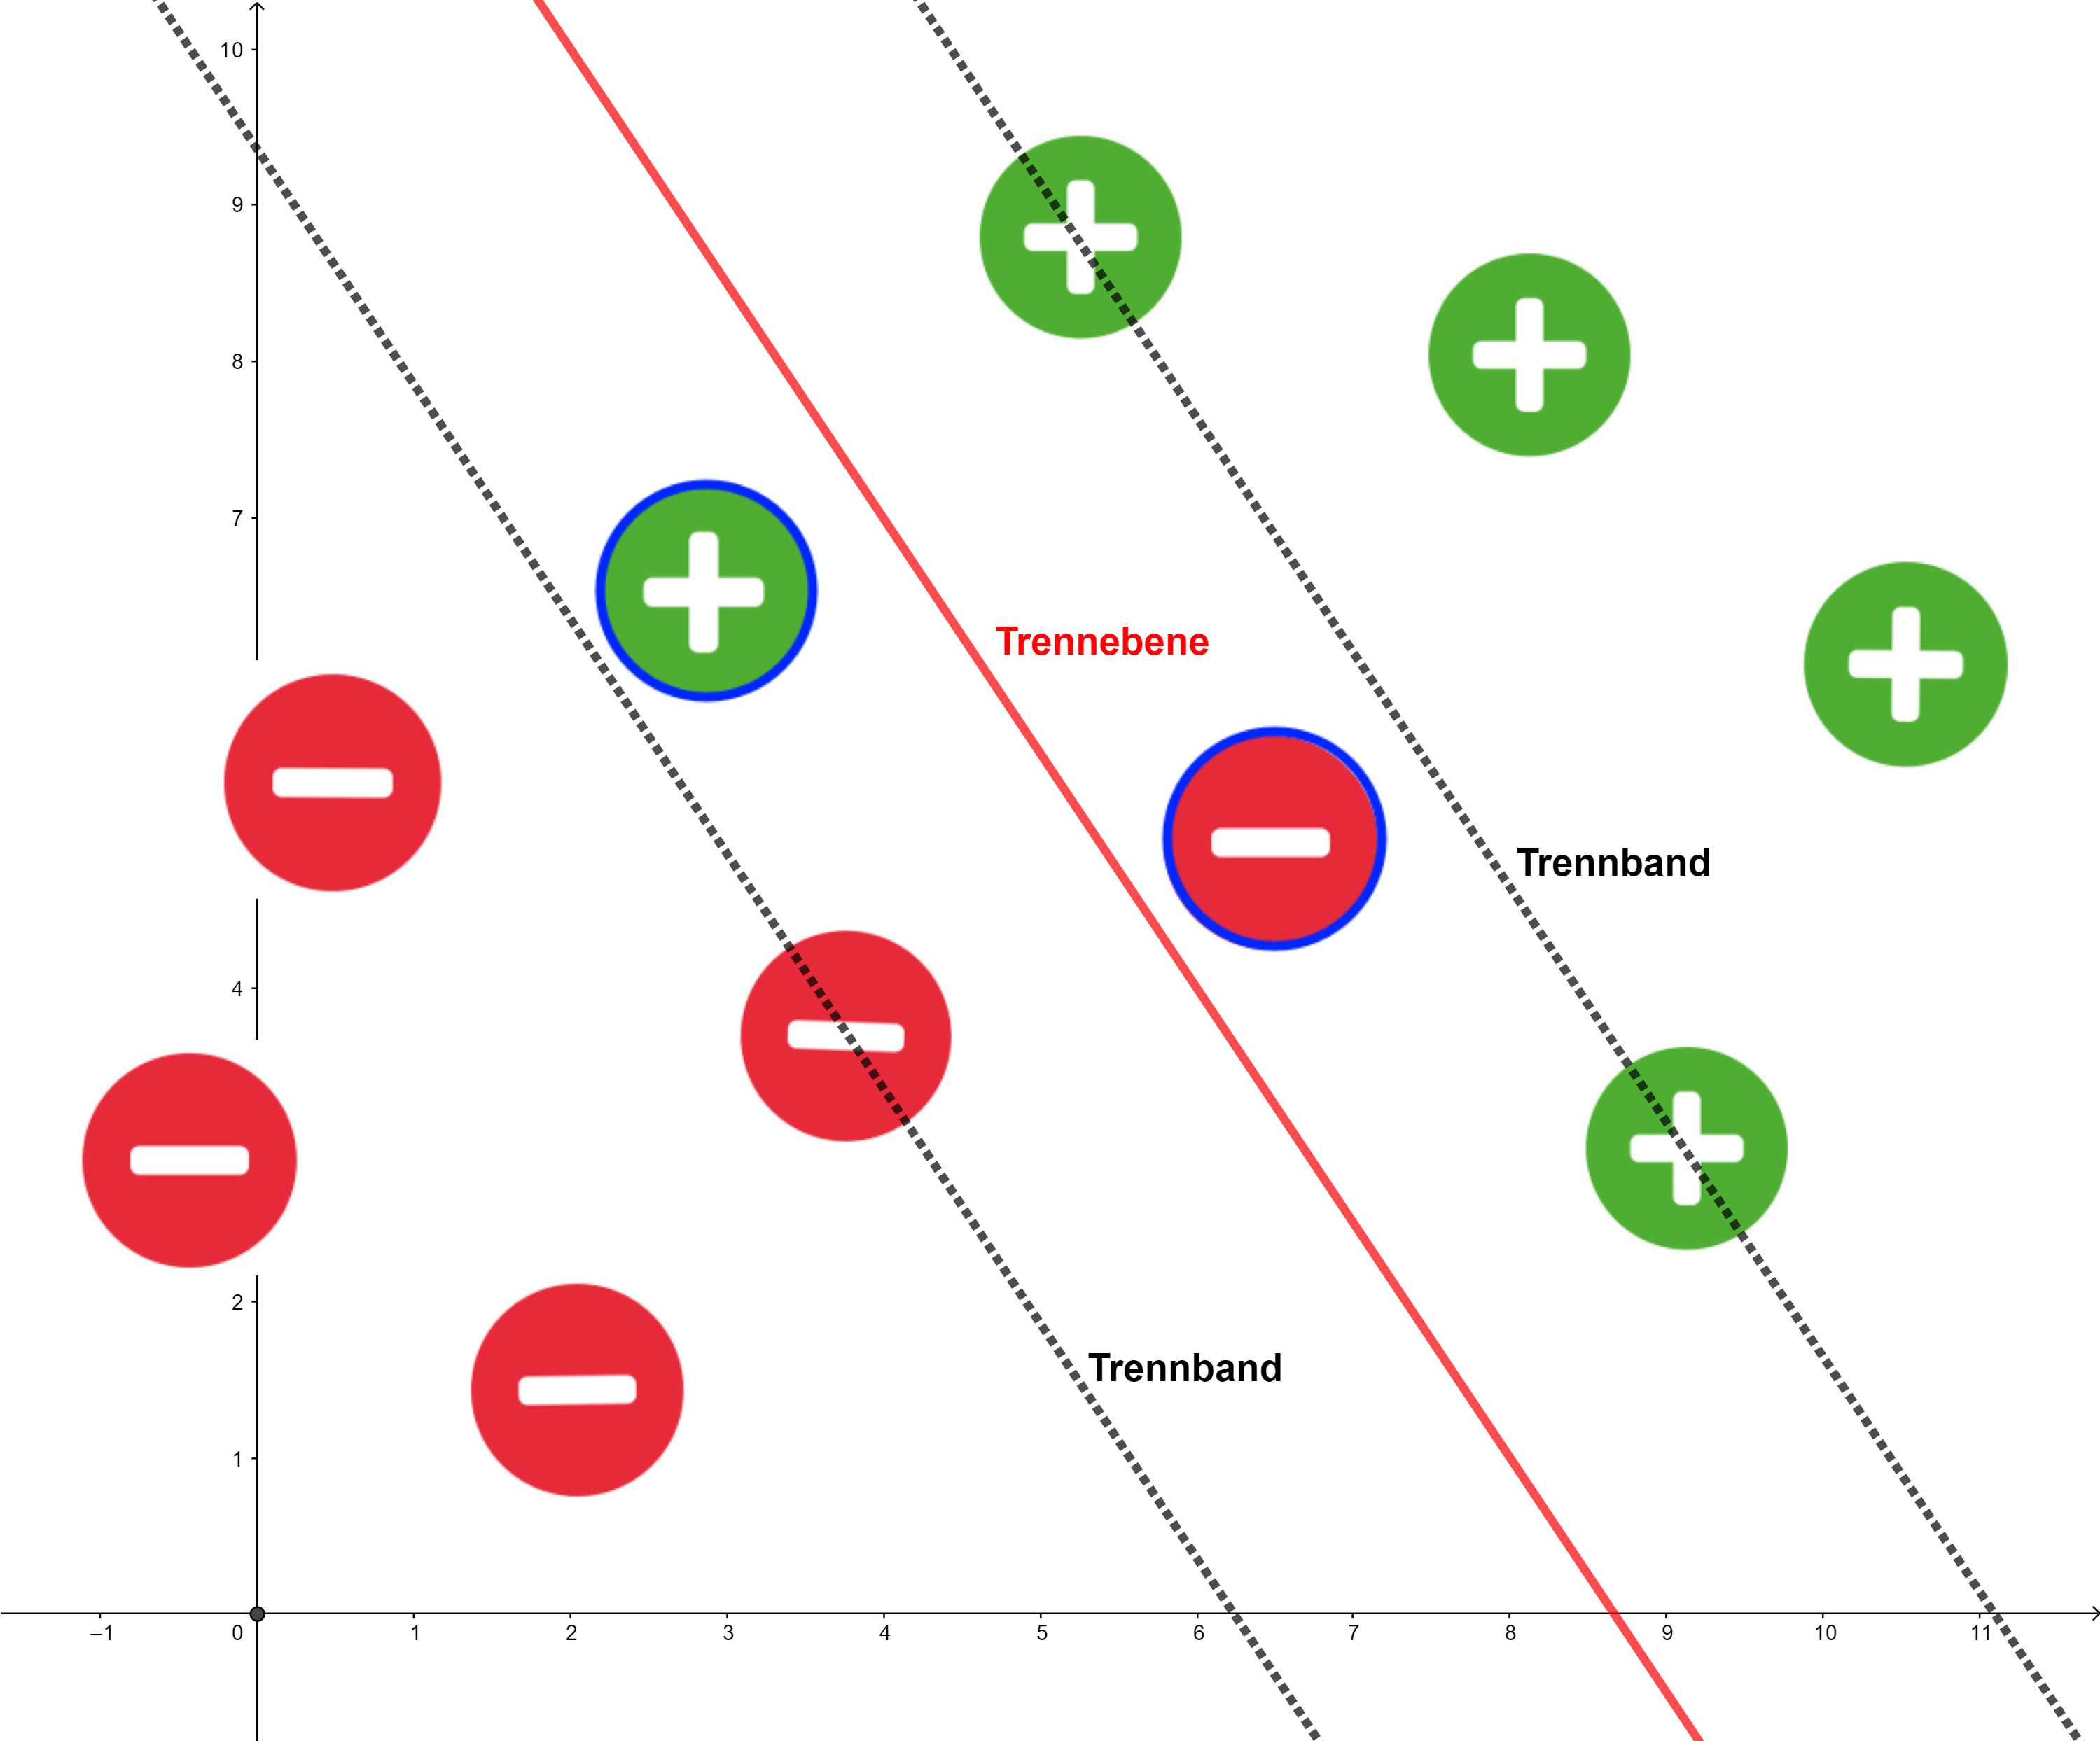
\includegraphics[width = 12cm]{assets/soft_margin_example.png}
	\caption{Die Eingabevektoren können nicht ohne einzelne Fehlklassifizierungen (blau markiert) linear getrennt werden.}
	\label{fig:soft_margin_example}
\end{figure}

In den Überlegungen in \autoref{sec:hard_margin} wurde angenommen, dass alle Eingabevektoren linear separierbar sind ohne dass Fehlklassifikationen aufreten. Dieses Problem kann durch eine Hard-Margin \ac{SVM}, wie in den Kapiteln zuvor gezeigt, gelöst werden. Trifft diese Annahme für eine Menge von Eingabevektoren nicht mehr zu, wie in \autoref{fig:soft_margin_example} dargestellt, kann der bisher beschriebene Algorithmus keine lineare Trennebene finden. Durch die Einführung von positiven Fehlervariablen $\xi_{n} \in \mathbb{R}^{K}, \xi_{n} \geq 0$ in \autoref{decision_rules} kann dieses Problem umgangen werden und trotzdem eine fehlerbehaftete, lineare Trennebene gefunden werden:

\begin{subequations} \label{decision_rules_softmargin}
	\begin{alignat}{2}
		w^{T} x_{n} + b \geq +1 - \xi_{n}& \qquad & \text{ für } y_{n} = +1\\
		w^{T} x_{n} + b \leq -1 + \xi_{n}& & \text{ für } y_{n} = -1
	\end{alignat}
\end{subequations}


Damit ein Eingabevektor $x_{n}$ nun, gemäß \autoref{decision_rules_softmargin}, falsch klassifiziert werden kann muss der zu dem Vektor gehörende Fehler $\xi_{n}$ über $1$ steigen. Eine obere Grenze für die Anzahl der aufgetretenen Fehler kann somit beschrieben werden durch $\sum_{n=1}^{N} \xi_{n}$. \\

Basierend auf dieser Grundlage kann eine Kostenfunktion $E$ basierend auf der Anzahl der Fehler formuliert werden:
\begin{equation} \label{soft_margin_error_cost_function}
	\begin{aligned}
		E = C(\sum_{n=1}^{N} \xi_{n})
	\end{aligned}
\end{equation}

Der Parameter $C \in \mathbb{R}, C \geq 0$ bestimmt die Höhe der Bestrafung von Fehlern und kann frei gewählt werden. \\


Erweitert man die zu minimierende Funktion $\frac{1}{2} w^{T} w $ aus \autoref{min_problem} um die Kostenfunktion $C(\sum_{n=1}^{N} \xi_{n})$ so erhält man ein neues Optimierungsproblem:

\begin{subequations} \label{soft_margin_problem}
	\begin{alignat}{2}
		&\!\min_{w}        &\qquad&  \frac{1}{2} w^{T} w + C(\sum_{n=1}^{N} \xi_{n}) \label{eq:optProbsoft}\\
		&\text{mit } &      & y_n (w^{T} x_{n} + b)-1 \geq 0 \text{ für } n=1..N \label{eq:constraintsoft}
	\end{alignat}
\end{subequations}

Wendet man die in \autoref{sec:lagrange} beschriebenen Schritte auf das in \autoref{soft_margin_problem} beschriebene Problem an erhält man folgendes Optimierungsproblem:

\begin{subequations} \label{final_lagrange_soft}
	\begin{alignat}{2}
		&\!\max_{\alpha}        &\qquad&  	\Lagr(\alpha) = \sum_{n=1}^{N} \alpha_{n} - \frac{1}{2} \sum_{n=1}^{N} \sum_{m=1}^{M} y_{n} y_{m} \alpha_{n} \alpha_{m} x_{n}^{T} x_{m} \label{eq:soft_margin_final}\\
		&\text{mit } &      & 0 \leq \alpha_{n} \leq C \text{ für } n=1..N \label{eq:constraint_soft}\\
		&       & & \sum_{n=1}^{N} \alpha_{n} y_{n} = 0\text{ für } n=1..N
	\end{alignat}
\end{subequations}

Sehr bemerkenswert hier ist, dass der einzige Unterschied zu \autoref{final_lagrange} die Beschränkung der Lagrange Multiplikatoren durch $C$ ist. Umgekehrt bedeutet dies, dass eine Hard-Margin SVM durch \autoref{final_lagrange_soft} beschrieben werden kann wenn der Parameter $C$ sehr groß gewählt wird. \\

\chapter{Vergleich Soft-Margin und Hard-Margin Support Vector Machine}

Ein großer Vorteil der Soft-Margin \ac{SVM} ist die Verminderung des Einflusses von Ausreißern auf die Trenngrenze. Bei der Hard-Margin \ac{SVM} kann mitunter ein Ausreißer, der näher als alle anderen Punkte bei der anderen Klasse liegt, die Lage der Trenngrenze bestimmen. Die so bestimmte Trenngrenze liegt mitunter viel näher bei der abzugrenzenden Klasse als eine optimale Trenngrenze liegen würde. Ein Beispiel für eine solche Situation ist in \autoref{fig:hard_vs_soft_svm} dargestellt. Die Soft-Margin \ac{SVM} hat die Möglichkeit Fehlklassifikationen zuzulassen und kann dadurch bessere liegende Trennebenen finden die zu stabileren Klassfikationsergebnissen für neue Daten führt.\\

Aufgrund des zuvor genannten Verhaltens tendiert die Hard-Margin \ac{SVM} im Allgemeinen zu Overfitting. Aus diesem Grund sollte die Soft-Margin \ac{SVM} bevorzugt werden und der Parameter $C$ abhängig von den gegebenen Trainingsdaten gewählt werden.


\begin{figure}[H]
	\centering
	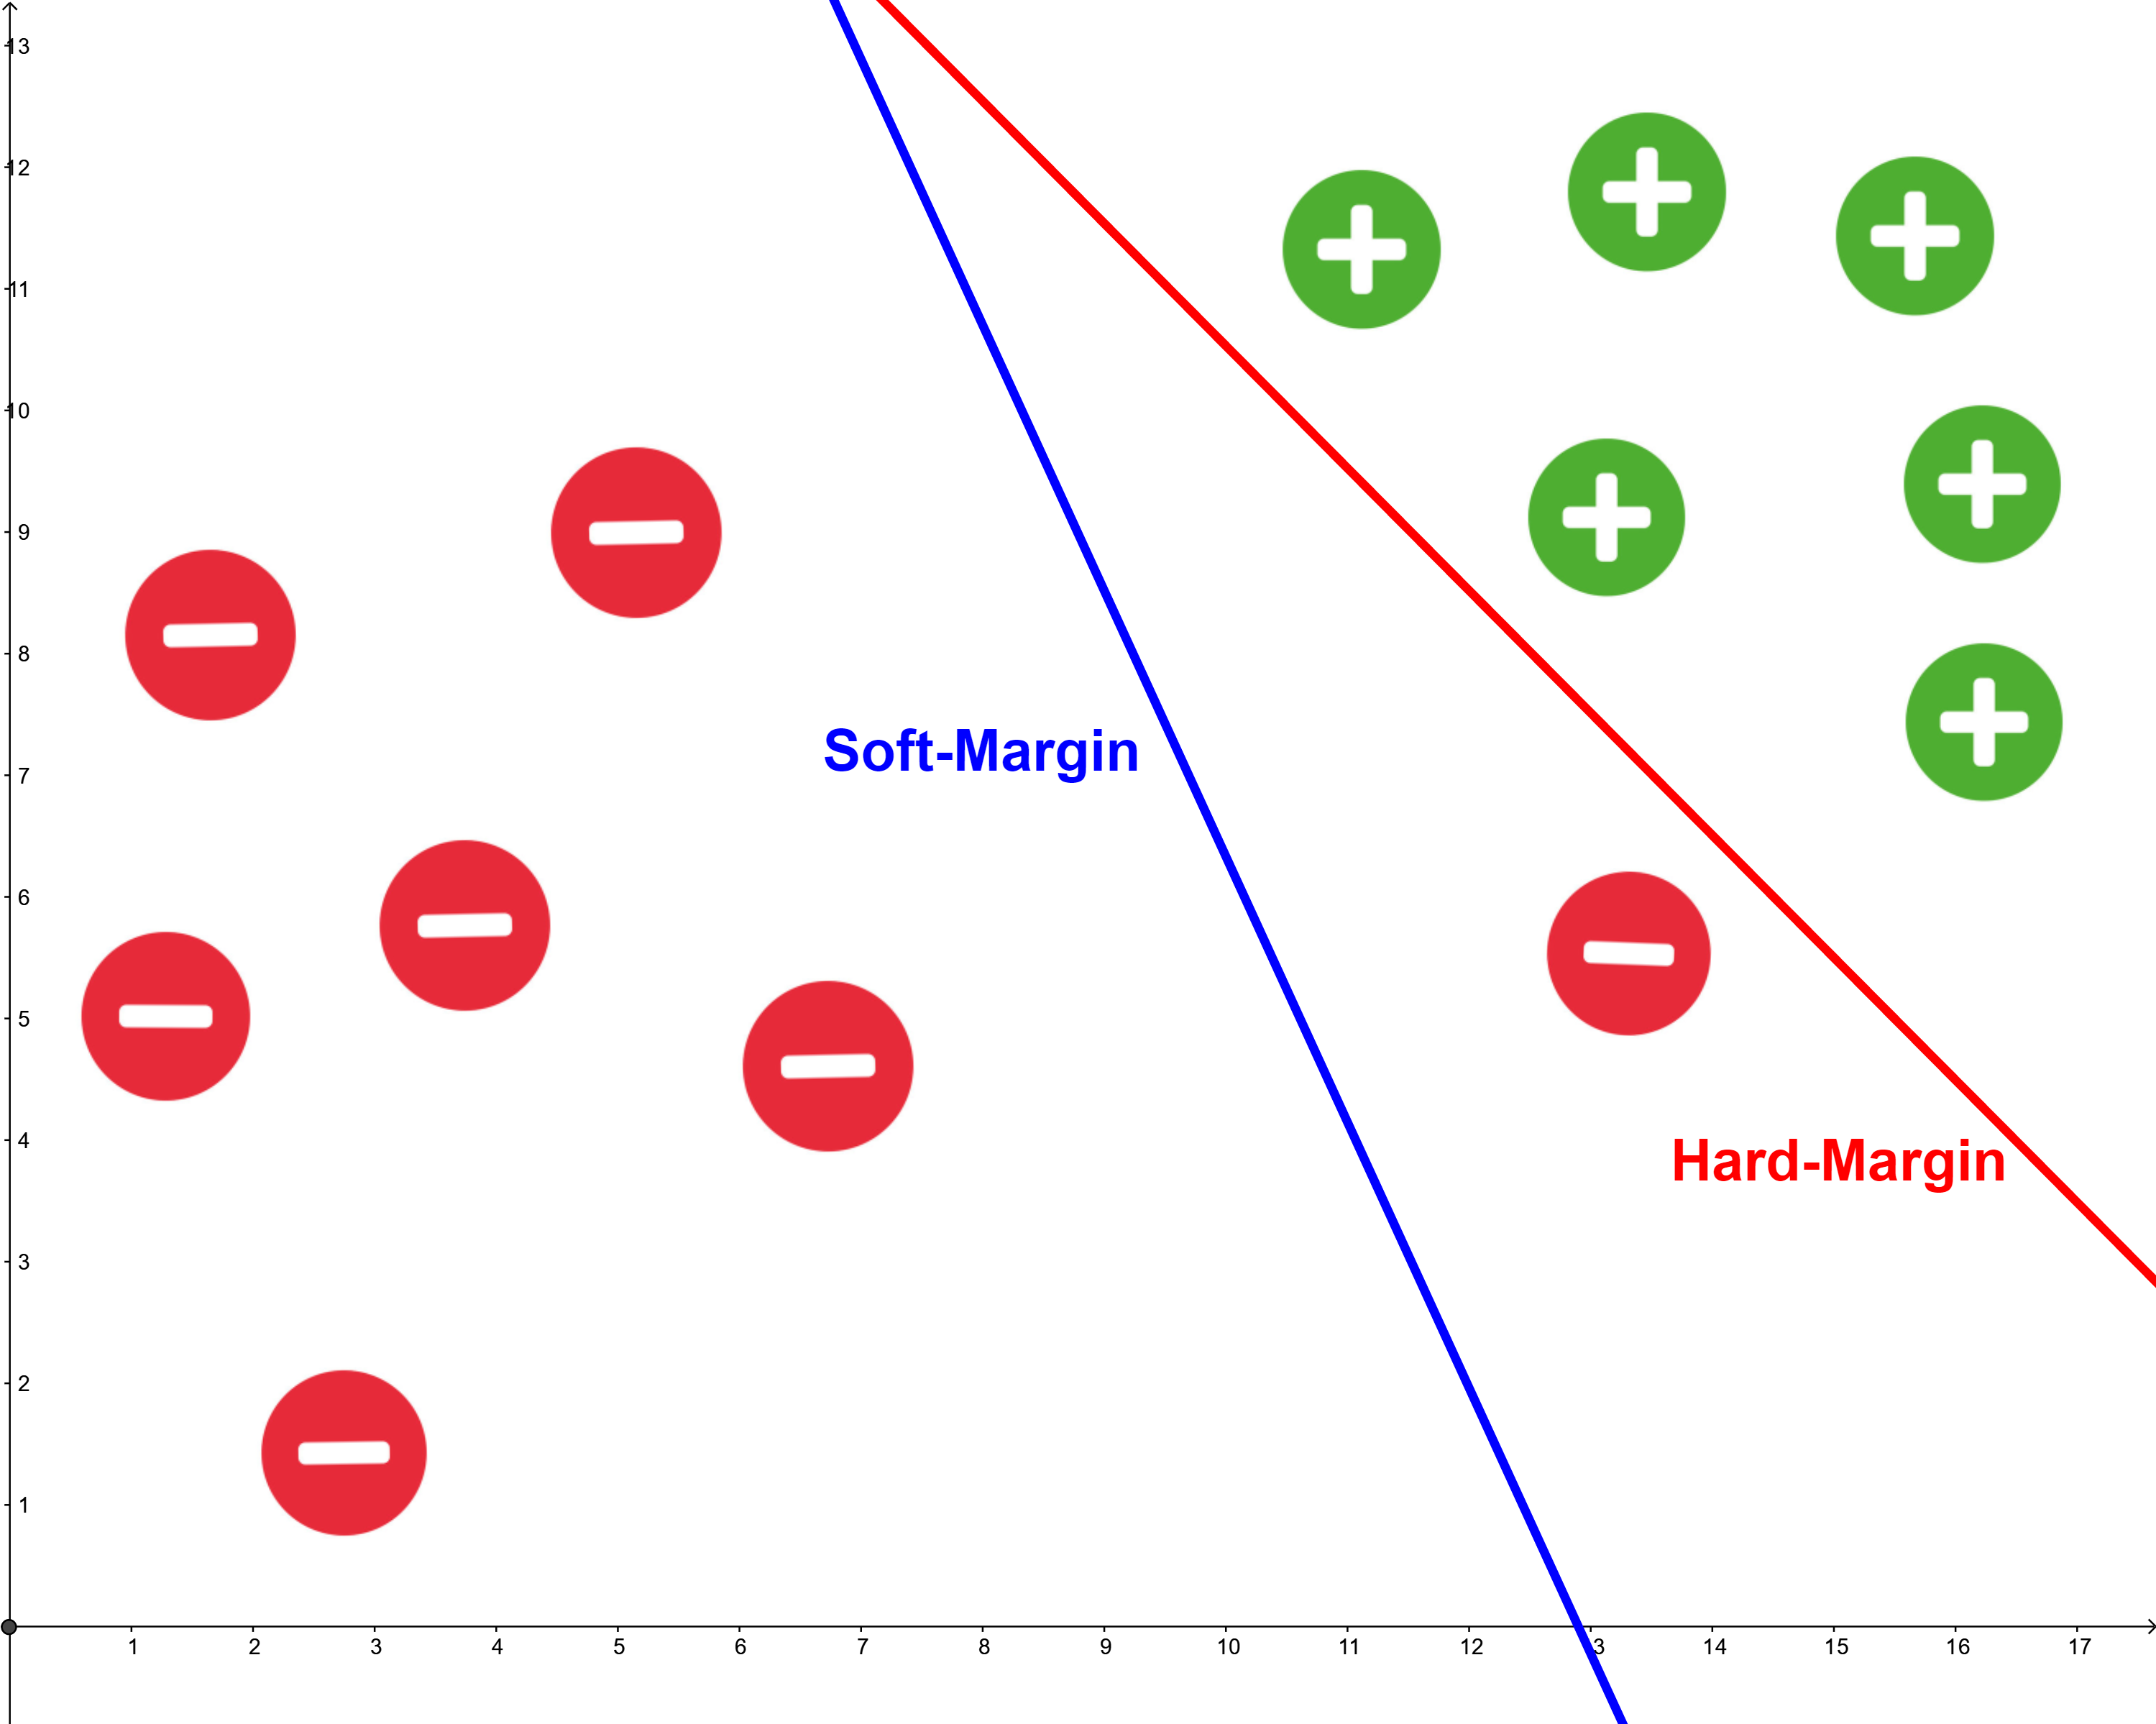
\includegraphics[width = 13cm]{assets/hard_vs_soft_margin.png}
	\caption{Die Hard-Margin \ac{SVM} trennt die Klassen zwar ohne Fehler, die Lage der Trennebene ist allerdings sehr nahe bei den grünen Punkten. Dadurch werden neue Eingabevektoren, die nahe bei der Trenngrenze liegen, mit großer Wahrscheinlichkeit falsch klassifiziert. Die Soft-Margin SVM \glqq{}opfert\grqq{} eine Fehlklassifikation für eine viel bessere, stabilere Lage der Trenngrenze.}
	\label{fig:hard_vs_soft_svm}
\end{figure}






\chapter{Nichtlineare Trennung}

Wird eine nichtlineare Trennung von Eingabevektoren gewünscht lässt sich dies nicht direkt durch eine \ac{SVM} realisieren, da eine \ac{SVM} in ihrer Grundform ausschließlich linear trennen kann. Werden die Eingabevektoren allerdings mittels einer Funktion so transformiert, dass diese linear trennbar sind, kann eine \ac{SVM} auch nichtlinear trennbare Eingabevektoren trennen. In \autoref{transform_phi} wird zuerst eine Intuition für die Transformation aufgebaut. Diese Intuition wird anschließend in \autoref{sec:kernel} weiter formalisiert und verallgemeinert. 

\section{Transformation der Problemstellung} \label{transform_phi}

Sind die Eingabevektoren nicht linear trennbar können diese mittels einer Transformation $\Phi(x): \mathbb{R}^{K} \rightarrow \mathbb{R}^{L}$ in einen Raum, in dem diese trennbar sind, transformiert werden. Beispiele für solche Transformationen sind in \autoref{fig:phi_transformation1} und \autoref{fig:phi_transformation2} dargestellt.


\begin{figure}[H]
	\centering
	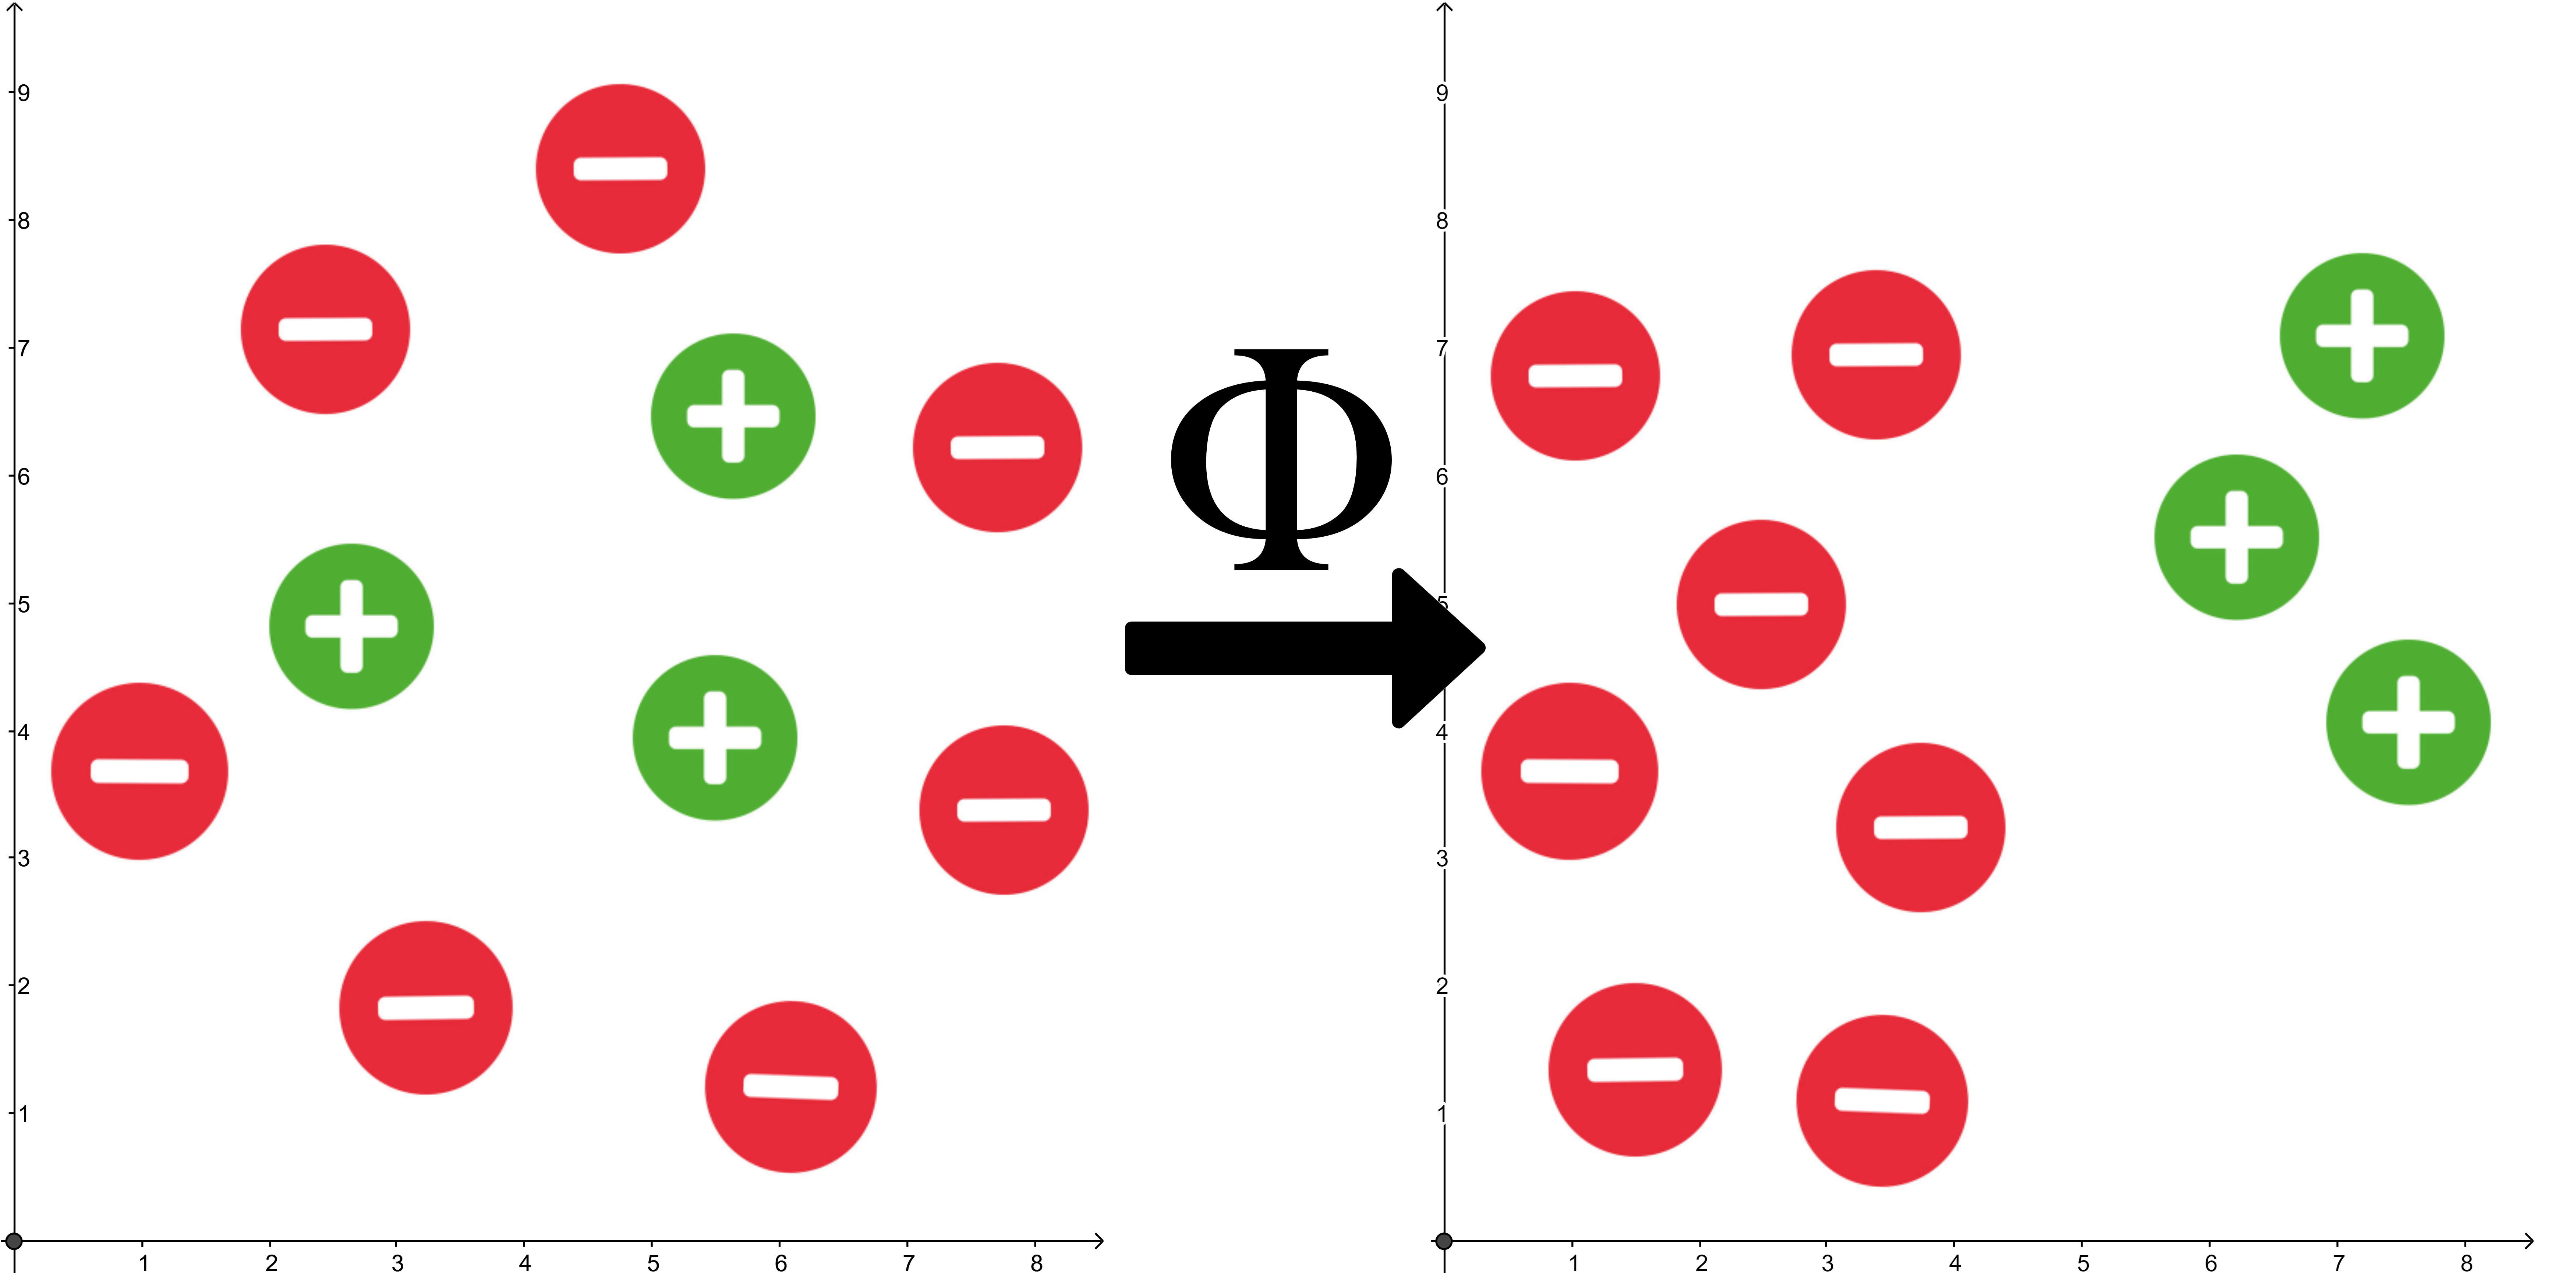
\includegraphics[width = 13cm]{assets/transformation.png}
	\caption{Die Eingabevektoren werden mittels einer Funktion $\Phi(x)$ transformiert. Die transformierten Vektoren sind linear trennbar.}
	\label{fig:phi_transformation1}
\end{figure}

\begin{figure}[H]
	\centering
	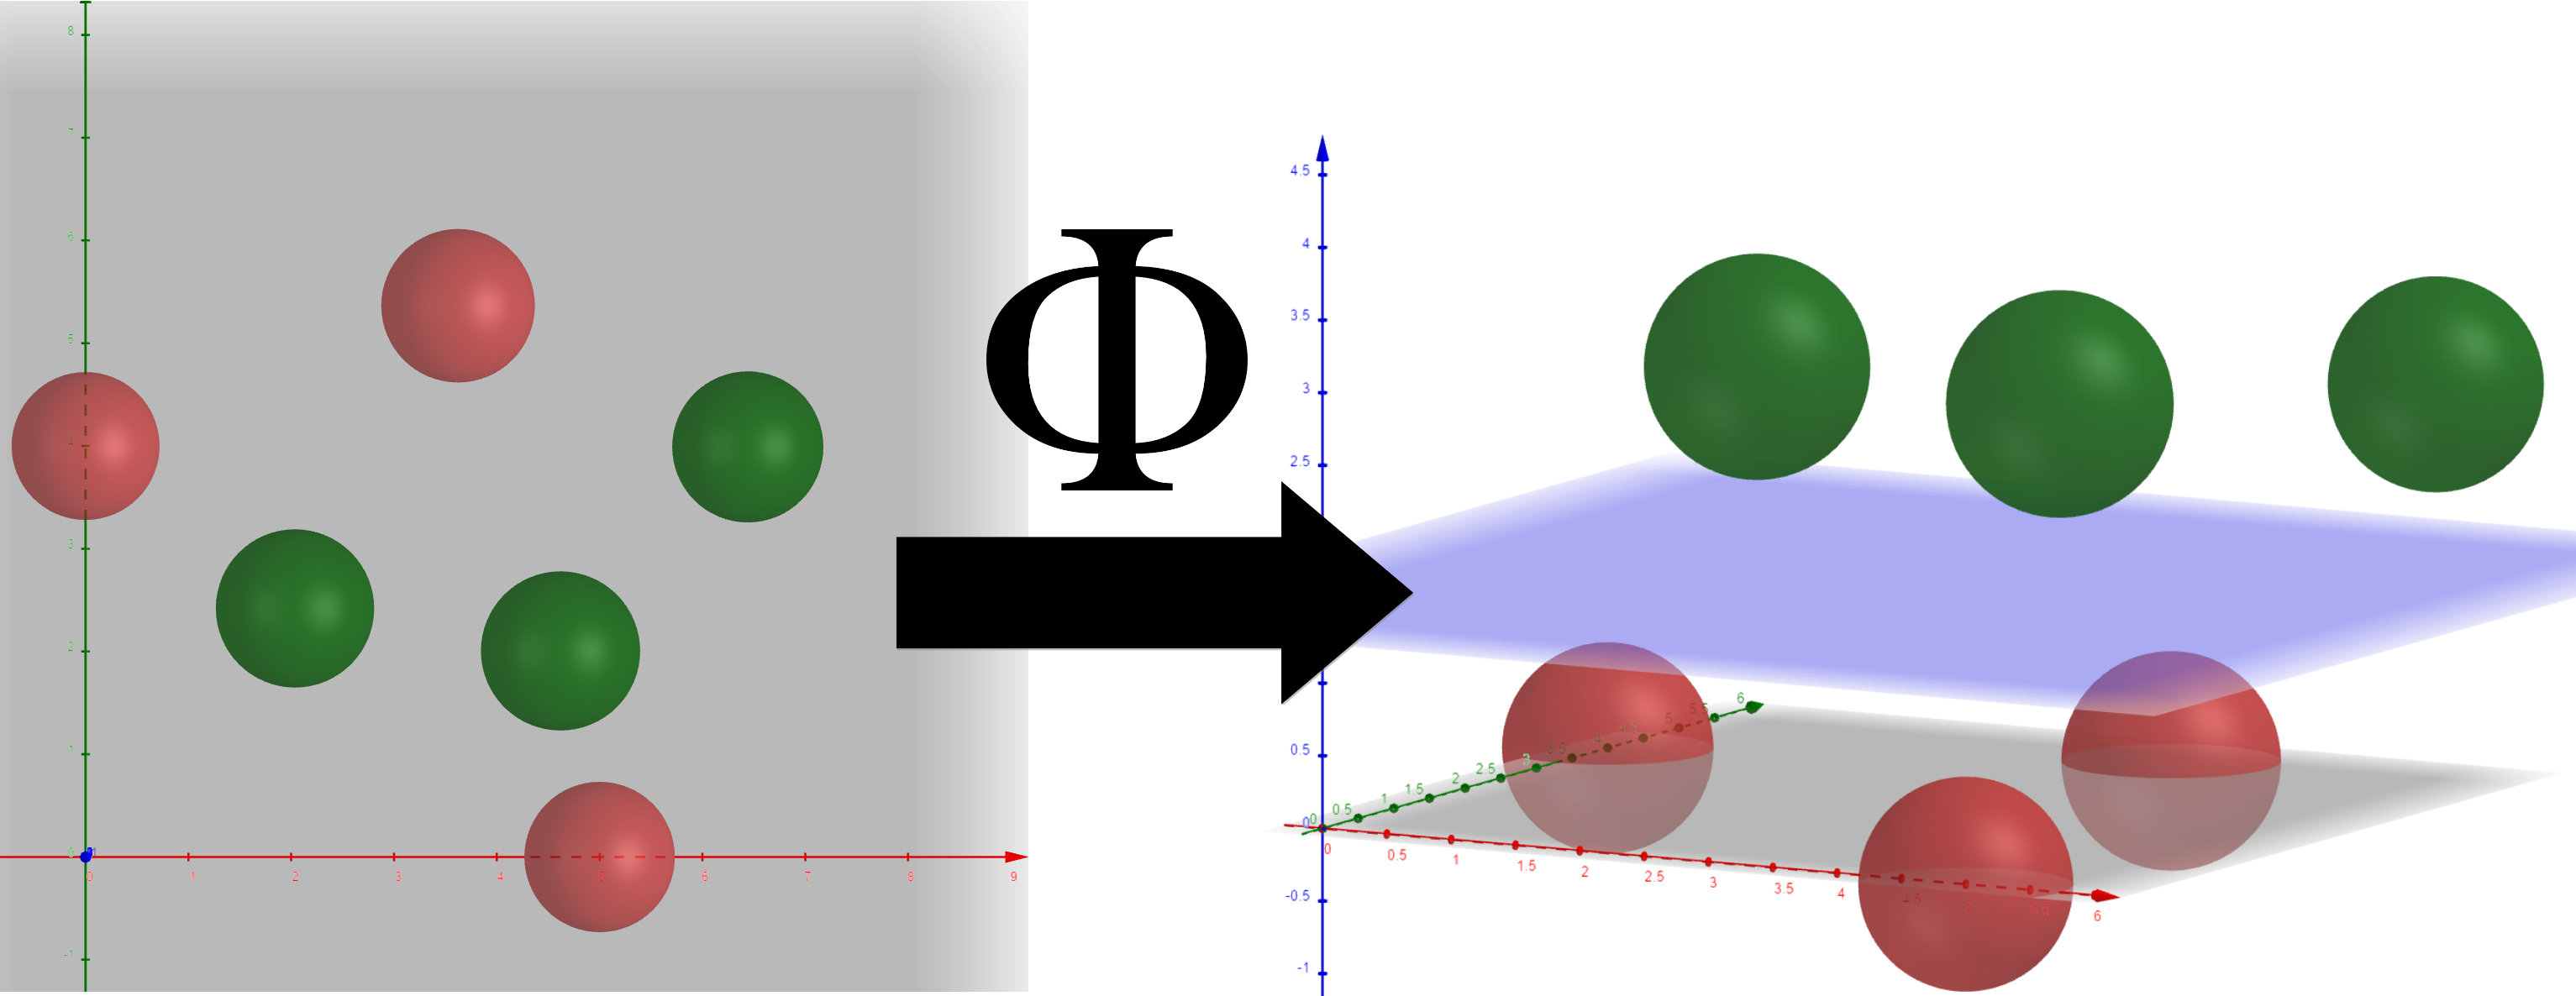
\includegraphics[width = 13cm]{assets/2d_to_3d_phi.png}
	\caption{Die Eingabevektoren werden mittels einer Funktion $\Phi(x)$ in einen höherdimensionalen Raum transformiert. Die transformierten Vektoren sind durch eine Ebene linear trennbar.}
	\label{fig:phi_transformation2}
\end{figure}



Wird statt allen Eingabevektoren $x$ deren transformierte Vektoren $\Phi(x)$ in \autoref{final_lagrange_soft} eingesetzt erhält man: 

\begin{subequations} \label{eq:soft_margin_with_transform}
	\begin{alignat}{2}
		&\!\max_{\alpha}        &\qquad&  	\Lagr(\alpha) = \sum_{n=1}^{N} \alpha_{n} - \frac{1}{2} \sum_{n=1}^{N} \sum_{m=1}^{M} y_{n} y_{m} \alpha_{n} \alpha_{m} \Phi(x_{n})^{T} \Phi(x_{m})\\
		&\text{mit } &      & 0 \leq \alpha_{n} \leq C \text{ für } n=1..N\\
		&       & & \sum_{n=1}^{N} \alpha_{n} y_{n} = 0\text{ für } n=1..N
	\end{alignat}
\end{subequations}

Wie in \autoref{eq:soft_margin_with_transform} ersichtlich sind die einzigen Zusatzkosten gegenüber einer Soft-Margin \ac{SVM} die Berechnungen der mitunter höherdimensionalen Skalarprodukte $\Phi(x)^{T} \Phi(x)$. Die Anzahl der Lagrangefaktoren $\alpha$ und die Dimension der Q-Matrix aus \autoref{qp1} bleibt gleich weil diese nur von der Anzahl der Eingabevektoren und nicht von der Dimension derer abhängig sind. \\

Die Stützvektoren dieser Methode befinden sich in dem neuen Raum $\mathbb{R}^{L}$, weil auch nur die transformierten Eingabevektoren betrachtet werden. Durch die, mitunter nichtlineare, Transformation $\Phi$ ist es so möglich mittels einer \ac{SVM} nichtlineare Trennungen durchführen zu können. \\

Das Problem dieses Ansatzes ist die Wahl der Transformationsfunktion $\Phi(x)$. Im Normalfall ist eine solche Funktion nicht bekannt. Trotzdem ist die Erkenntnis, dass die Dimension der Vektoren das Optimierungsproblem nicht groß beeinflusst und dass durch eine Transformation nichtlineare Trenngrenzen bestimmt werden können, äußerst relevant für die weitere Betrachtung. In \autoref{sec:kernel} wird beschrieben wie die Zusatzkosten der Skalarprodukte auch umgangen werden können.

\section{Kernel Trick} \label{sec:kernel}

Wie in \autoref{transform_phi} beschrieben können die Eingabevektoren mittels einer Funktion $\Phi$ in einen anderen, beliebigen Raum transformiert werden. In diesem Kapitel wird diese Idee der Transformation verallgemeinert betrachtet. \\

Für die Betrachtung wird das Optimierungsproblem und die Formeln für $w$ und $b$ für die Soft-Margin \ac{SVM} so abgeändert, dass statt allen Eingabevektoren $x$ deren transformierte Form $z = \Phi(x)$ eingesetzt wird:

\begin{subequations} 
	\begin{alignat}{2}
		&\!\max_{\alpha}        &\qquad&  	\Lagr(\alpha) = \sum_{n=1}^{N} \alpha_{n} - \frac{1}{2} \sum_{n=1}^{N} \sum_{m=1}^{M} y_{n} y_{m} \alpha_{n} \alpha_{m} z_{n}^{T} z_{m}\\
		&\text{mit } &      & 0 \leq \alpha_{n} \leq C \text{ für } n=1..N\\
		&       & & \sum_{n=1}^{N} \alpha_{n} y_{n} = 0\text{ für } n=1..N
	\end{alignat}
\end{subequations}

Für die Berechnung von $w$ und $b$ ergibt sich:
\begin{equation}
	\begin{aligned}
		w &= \sum_{n=1}^{N} \alpha_{n} y_{n} z_{n}
	\end{aligned}
\end{equation}

\begin{equation}
	\begin{aligned}
		b &= \frac{1}{y_{k}} - w^{T} z_{k}
	\end{aligned}
\end{equation}

Wie bereits zuvor erwähnt hängt das Problem ausschließlich von den Skalarprodukten der Eingabevektoren, die jetzt in ihrer transformierten Form verwendet werden, ab. Werden die Eingabevektoren mittels $\Phi$ in einen sehr hochdimensionalen, mitunter unendlich dimensionalen, Raum transformiert kann die Berechnung des Skalarprodukts sehr aufwändig bis gar nicht berechnbar werden. \\

Durch die Einführung einer Kernel-Funktion $K(x, x') = z_{1}^{T} z_{2} = \Phi(x)^{T} \Phi(x')$, die das Skalarprodukt der transformierten Eingabevektoren berechnet ohne die Eingabevektoren tatsächlich in den neuen Raum zu transformieren, kann das Problem der Berechnung von hochdimensionalen Skalarprodukten umgangen werden. \\


\subsection{Beispiel Kernel-Funktion} \label{sec:example_kernel}
Die Idee einer Kernel-Funktion wird nun anhand eines einfachen Beispiels gezeigt. Folgende Kernel-Funktion für $x, x' \in \mathbb{R}^2$ sei gegeben:

\begin{equation} \label{eq:example1_kernel}
	\begin{aligned}
		K(x, x') &= (1 + x^{T}x')^{2} = \\
		&= (1 + x_{1} x_{1}' + x_{2} x_{2}')^{2} = \\
		&= 1 + x_{1}^2 x_{1}'^2 + x_{2}^{2} x_{2}'^{2} + 2x_{1} x_{1}' + 2 x_{2} x_{2}' + 2 x_{1} x_{1}'x_{2} x_{2}'
	\end{aligned}
\end{equation}

Diese Kernel-Funktion scheint auf den ersten Blick nicht, wie zuvor definiert, einem Skalarprodukt der transformierten Vektoren $\Phi(x)$ und $\Phi(x')$ zu entsprechen.\\
 
Angenommen die verwendete Transformationsfunktion $\Phi$ entspräche:

\begin{equation}
	\begin{aligned}
		\Phi(x) &= (1, x_{1}^{2}, x_{2}^{2}, \sqrt{2} x_{1}, \sqrt{2} x_{2}, \sqrt{2} x_{1} x_{2})\\
	\end{aligned}
\end{equation}

Angewandt auf die Vektoren $x$ und $x'$:
\begin{equation} \label{eq:example1_innerprod}
	\begin{aligned}
		\Phi(x) &= (1, x_{1}^{2}, x_{2}^{2}, \sqrt{2} x_{1}, \sqrt{2} x_{2}, \sqrt{2} x_{1} x_{2})\\
		\Phi(x') &= (1, x_{1}'^{2}, x_{2}'^{2}, \sqrt{2} x_{1}', \sqrt{2} x_{2}', \sqrt{2} x_{1}' x_{2}')\\
		\Phi(x)^T \Phi(x') &= 1 + x_{1}^2 x_{1}'^2 + x_{2}^{2} x_{2}'^{2} + 2x_{1} x_{1}' + 2 x_{2} x_{2}' + 2 x_{1} x_{1}'x_{2} x_{2}'
	\end{aligned}
\end{equation}

Werden die Ergebnisse von \autoref{eq:example1_kernel} und \autoref{eq:example1_innerprod} verglichen erkennt man, dass die Kernel-Funktion $(1 + x^{T}x')^{2}$ tatsächlich dem Skalarprodukt der mit $\Phi$ transformierten Vektoren $x$ und $x'$ entspricht. \\

$\Phi$ transformiert in diesem Beispiel 2-dimensionale Vektoren nach $\mathbb{R}^6$. Mittels der Kernel-Funktion kann das Skalarprodukt der transformierten Vektoren durch $K(x, x') = (1 + x^{T}x')^{2}$ berechnet werden ohne dass die Vektoren $x$ und $x'$ tatsächlich in den neuen Raum transformiert werden müssen. \\

In dem Beispiel wurde die Berechnung von 6-dimensionalen Skalarprodukten durchgeführt durch die Berechnung mittels der Kernel-Funktion, die lediglich 2-dimensionale Skalarprodukte berechnen muss. Führt die Funktion $\Phi$ eine Transformation in eine viel höhere oder unendlich hohe Dimension aus ist der Vorteil einer solchen Kernel-Funktion sofort ersichtlich.

\subsection{Polynomieller Kernel}
Die in \autoref{sec:example_kernel} verwendete Kernel-Funktion kann verallgemeinert werden. Seien die Eingabevektoren $x \in \mathbb{R}^d$ und die Transformationsfunktion $\Phi: \mathbb{R}^d \rightarrow \mathbb{Z}$ ein Polynom der Ordnung $Q$, dann kann eine Kernel-Funktion wie folgt definiert werden:

\begin{equation} \label{eq:poly_kernel}
	\begin{aligned}
		K(x, x') &= (1 + x^{T}x')^{Q} = \\
		&= (1 + x_{1} x_{1}' + x_{2} x_{2}' + \dots + x_{d} x_{d}')^{Q}
	\end{aligned}
\end{equation}

Die in \autoref{eq:poly_kernel} beschriebene Kernel-Funktion wird polynomieller Kernel genannt. Weil durch das Polynom eine Vielzahl an Faktoren entsteht kann zur Kompensation dieser Faktoren die Kernel-Funktion mit den Skalierungsfaktoren $a$ und $b$ erweitert werden:

  \begin{equation} \label{eq:poly_kernel2}
  	\begin{aligned}
  		K(x, x') &= (a x^{T}x' + b)^{Q}
  	\end{aligned}
  \end{equation}

Mittels dieser Kernel-Funktion kann die Berechnung eines Skalarprodukts eines beliebig großen Polynoms des Grades $Q$ durch die Berechnung eines Skalarprodukts in $\mathbb{R}^{d}$ und der Exponentation mit $Q$ durchgeführt werden ohne dass die Vektoren tatsächlich in den Polynomraum transformiert werden müssen.  

\subsection{Radial Basis Function Kernel}

Eine weitere mögliche Kernel-Funktion ist der \ac{RBF} Kernel:
\begin{equation} \label{eq:rbfk}
	\begin{aligned}
		K(x, x') &= \exp{\gamma \norm{x - x'}^2}
	\end{aligned}
\end{equation}

Hierbei ist $\gamma$ ein frei wählbarer Parameter.
Die zu diesem Kernel zugehörige Transformationsfunktion $\Phi$ bildet in einen unendlich dimensionalen Raum ab.
Dies kann wie folgt gezeigt werden (für den einfachsten Fall):

\begin{equation} \label{eq:proof_rbfk_infinite}
	\begin{aligned}
		K(x, x') &= \exp{(-(x - x')^{2})} =\\
		&= \exp{(-x^{2} + 2xx' - x'^{2})} = \\
		&= \exp{(-x^{2})} \exp{(2xx')} \exp{(-x'^{2})} = \\
		&= \exp{(-x^{2})} \sum_{k=0}^{\infty} \frac{2^{k} (x)^{k} (x')^{k}}{k!} \exp{(-x'^{2})}
	\end{aligned}
\end{equation}

Durch die Taylorexpansion von $\exp{(2xx')}$ wird die Unendlichkeit dieses Raums sichtbar. Das Ergebnis von \autoref{eq:proof_rbfk_infinite} hat bereits die für ein Skalarprodukt benötigte Symmetrie von $exp(-x^{2})$ - $exp(-x'^{2})$ und $(x)^{k}$ - $(x')^{k}$. Die Anteile $\frac{2^k}{k!}$ können gleichmäßig auf $x$ und $x'$ aufgeteilt werden indem je die Wurzel der Anteile zu $x$ und $x'$ multipliziert werden. Damit wurde gezeigt dass der \ac{RBF} Kernel das Skalarprodukt in einem unendlich dimensionalen Raum berechnet. 

\subsection{SVM Definition mit Kernel}
Ein Input $x$, transformiert mit einer Funktion $z = \Phi(x)$, kann mit einer \ac{SVM} wie folgt klassifiziert werden:

\begin{equation} \label{eq:svm_def_kernel}
	\begin{aligned}
		y(x) &= sign(w^{T} z + b)
	\end{aligned}
\end{equation}

Diese Definition setzt voraus, dass die Funktion $\Phi$ bekannt ist. Das Ziel der neuen Definition ist die Vermeidung von einzeln auftretenden transformierten Eingabevektoren $z$ in den Formeln um das gesamte Problem mittels einer Kernel-Funktion $K(x, x')$ ausdrücken zu können ohne die Funktion $\Phi$ tatsächlich kennen zu müssen.

\begin{equation} \label{eq:kernel_w}
	\begin{aligned}
		w &= \sum_{z_{n} \text{ ist SV}} \alpha_{n} y_{n} z_{n}
	\end{aligned}
\end{equation}

Setzt man \autoref{eq:kernel_w} in \autoref{eq:svm_def_kernel} ein erhält man:

\begin{equation} \label{eq:svm_def_kernel2}
	\begin{aligned}
		y(x) &= sign(\sum_{\alpha_{n} > 0} \alpha_{n} y_{n} z_{n}^{T} z + b) = \\
		&= sign(\sum_{\alpha_{n} > 0} \alpha_{n} y_{n} K(x_{n}, x) + b)
	\end{aligned}
\end{equation}

Für $b$ ergibt sich durh Einsetzen von \autoref{eq:kernel_w} für einen beliebigen Stützvektor $x_{k}$:

\begin{equation}
	\begin{aligned}
		b &= \frac{1}{y_{k}} - w^{T} z_{k} = \\
		&= \frac{1}{y_{k}} - \sum_{\alpha_{n} > 0} \alpha_{n} y_{n} K(x_{n}, x_{k}) = \\
		&= y_{k} - \sum_{\alpha_{n} > 0} \alpha_{n} y_{n} K(x_{n}, x_{k}) = \\
	\end{aligned}
\end{equation}

Die \ac{SVM} ist nun vollständig definiert durch die Verwendung der Kernel-Funktion ohne dass die Transformationsfunktion $\Phi$ bekannt sein muss. Es wird keine einzige tatsächliche Transformation eines Eingabevektors mittels $\Phi$ benötigt und es können beliebig dimensionale Räume durch die Verwendung von entsprechenden Kernel-Funktionen verwendet werden. \\

Da die Funktion $\Phi$ überhaupt nicht bekannt sein muss impliziert das, dass beliebige Kernel-Funktionen verwendet werden können. Das ist in der Tat möglich, allerdings müssen die Kernel-Funktionen bestimmte Eigenschaften erfüllen. Diese werden in \autoref{sec:kernel_conditions} erläutert.\\

Das in \autoref{sec:qp} beschriebene Lösungsverfahren ist für das neue Problem nach wie vor gültig, lediglich die $Q$-Matrix muss entsprechend angepasst werden. Es muss nur statt $x_{n}^{T}x_{m}$ $K(x_{n}, x_{m})$ eingesetzt werden:

\begin{subequations} \label{qp1}
	\begin{alignat}{2}
		&\!\min_{\alpha}        &\qquad& \Lagr(\alpha) = \frac{1}{2} \alpha^{T} Q \alpha + (-1^T) \alpha \label{eq:qp1}\\
		&\text{mit} &      & Q = \begin{bmatrix} 
			y_{1}y_{1} K(x_{1}, x_{1}) & y_{1}y_{2} K(x_{1}, x_{2}) & \dots & y_{1}y_{N} K(x_{1}, x_{N})\\
			y_{2}y_{1} K(x_{2}, x_{1}) & y_{2}y_{2} K(x_{2}, x_{2}) & \dots & y_{2}y_{N} K(x_{2}, x_{N})\\
			\vdots & \vdots & \vdots & \vdots\\
			y_{N}y_{1} K(x_{N}, x_{1}) & y_{N}y_{2} K(x_{N}, x_{2}) & \dots & y_{N}y_{N} K(x_{N}, x_{N})\\ 
		\end{bmatrix}\\
		&\text{für} & & y^{T} \alpha = 0\\
		& & & 0 \leq \alpha \leq \infty
	\end{alignat}
\end{subequations} 

Mit dieser Änderung kann das Problem wieder an ein Quadratic Programming Framework übergeben werden um die $\alpha$ Werte zu bestimmen. Die \ac{SVM} lässt sich somit in Kombination mit Kernel-Funktionen auf beliebige binäre Klassifikationsprobleme anwenden. 


\subsection{Anforderungen an eine Kernel-Funktion} \label{sec:kernel_conditions}
Wie in den Kapiteln zuvor gezeigt wurde gibt es eine Vielzahl von verschiedenen Kernel-Funktionen. Wenn eine neue Funktion als Kernel-Funktion verwendet werden soll muss diese einem Skalarprodukt in einem Raum entsprechen. Um dies überprüfen zu können gibt es zwei verschiedene Ansätze:

\begin{itemize}
	\item Für eine vermutlich richtige Kernel-Funktion wird konstruktiv versucht die zugehörige Transformationsfunktion $\Phi$ zu bestimmen. Diese Vorgehensweise wurde in \autoref{sec:example_kernel} durchgeführt.
	
	\item Der Kernel $K(x, x')$ ist ein gültiger Kernel wenn die Funktion $K(x, x')$ symmetrisch ist und die Matrix \[ 	
	\begin{aligned}
		K &= 
		\begin{bmatrix} 
			K(x_{1}, x_{1}) & K(x_{1}, x_{2}) & \dots & K(x_{1}, x_{N})\\
			K(x_{2}, x_{1}) & K(x_{2}, x_{2}) & \dots & K(x_{2}, x_{N})\\
			\vdots & \vdots & \vdots & \vdots\\
			K(x_{N}, x_{1}) & K(x_{N}, x_{2}) & \dots & K(x_{N}, x_{N})\\ 
		\end{bmatrix}
	\end{aligned}
\] positiv semi-definit ist für jedes beliebige $x_1..x_N$. Die Forderung der positiv semi-definiten Matrix wird auch Satz von Mercer genannt und garantiert bei Erfüllung dass eine Funktion $\Phi$ existiert die in einen Raum abbildet dessen Skalarprodukte durch die Kernel-Funktion beschrieben werden können. 
\end{itemize}


\chapter{Pseudocode und Beispiele} \label{ch:pseudobsp}
In diesem Kapitel werden Pseudocodes von verschiedensten Varianten von SVMs präsentiert, von einer Hard-Margin \ac{SVM} bis zu einer Soft-Margin \ac{SVM} mit \ac{RBF}-Kernel.
Weiters werden anhand von Beispielen die Funktionsweisen und Eigenschaften der verschiedenen SVMs anschaulich demonstriert.

\section{Hard-Margin SVM Pseudocode}\label{sec:hsvmpseudo}
Es folgt der Pseudocode mit Anmerkungen für eine Hard-Margin Support Vector Machine.
\begin{table}[H]\label{tab:hmpc}
\begin{tabular}{|l r|}
    \hline
    \textbf{Hard-Margin SVM} & \textbf{Zeile} \\
    \hline
    Initialisiere $x, y$ & 1\\
    $Q = (yy^{\mathbf{T}})K$ & 2\\
    $c = \left( -1, -1, \ldots, -1 \right)^{\mathbf{T}}$ & 3 \\
    $A = diag\left( -1, -1, \ldots, -1 \right)$ & 4 \\
    $b = \left( 0, 0, \ldots, 0 \right)$ & 5\\
    $A_{eq} = Y^{\mathbf{T}}$ & 6\\
    $b_{eq} = 0$ & 7\\
    $\alpha = QPSolver\left( Q, c, A, b, A_{eq}, b_{eq} \right)$ & 8\\
    $w = \sum_{n=SV} \alpha_{n} y_{n} x_{n} $  & 9\\
    $b = \frac{1}{y_{n}} - w^{\mathbf{T}}x_{n}$ & 10\\
    \hline
\end{tabular}
\begin{tabular}{|l|}
    \hline
    \textbf{Anmerkungen} \\
    \hline
    Zeile 1: Initialisieren von Werte- und Klassenvektoren\\
    Zeile 2: Berechnen der Matrix Q \\
    Zeile 3: Berechnen von c \\
    Zeile 4, 5: Berechnen der Ungleichheitsbedingungen\\
    Zeile 6, 7: Berechnen der Gleichheitsbedingungen\\
    Zeile 8: Lösen mittels Quadratic Programming \\
    Zeile 9: Berechnung Gewichte mit Stützvektoren \\
    Zeile 10: Berechnung bias mit beliebigem Stützvektor \\
    \hline
\end{tabular}
\end{table}

\section{Hard-Margin SVM - Beispiel}\label{sec:hmsvmbsp}
Mit einer Hard-Margin \ac{SVM} können linear separierbare Punkte getrennt werden.
\autoref{fig:hmsvmbsp_simple} zeigt ein Beispiel.
\begin{figure}[H]
    \centering
    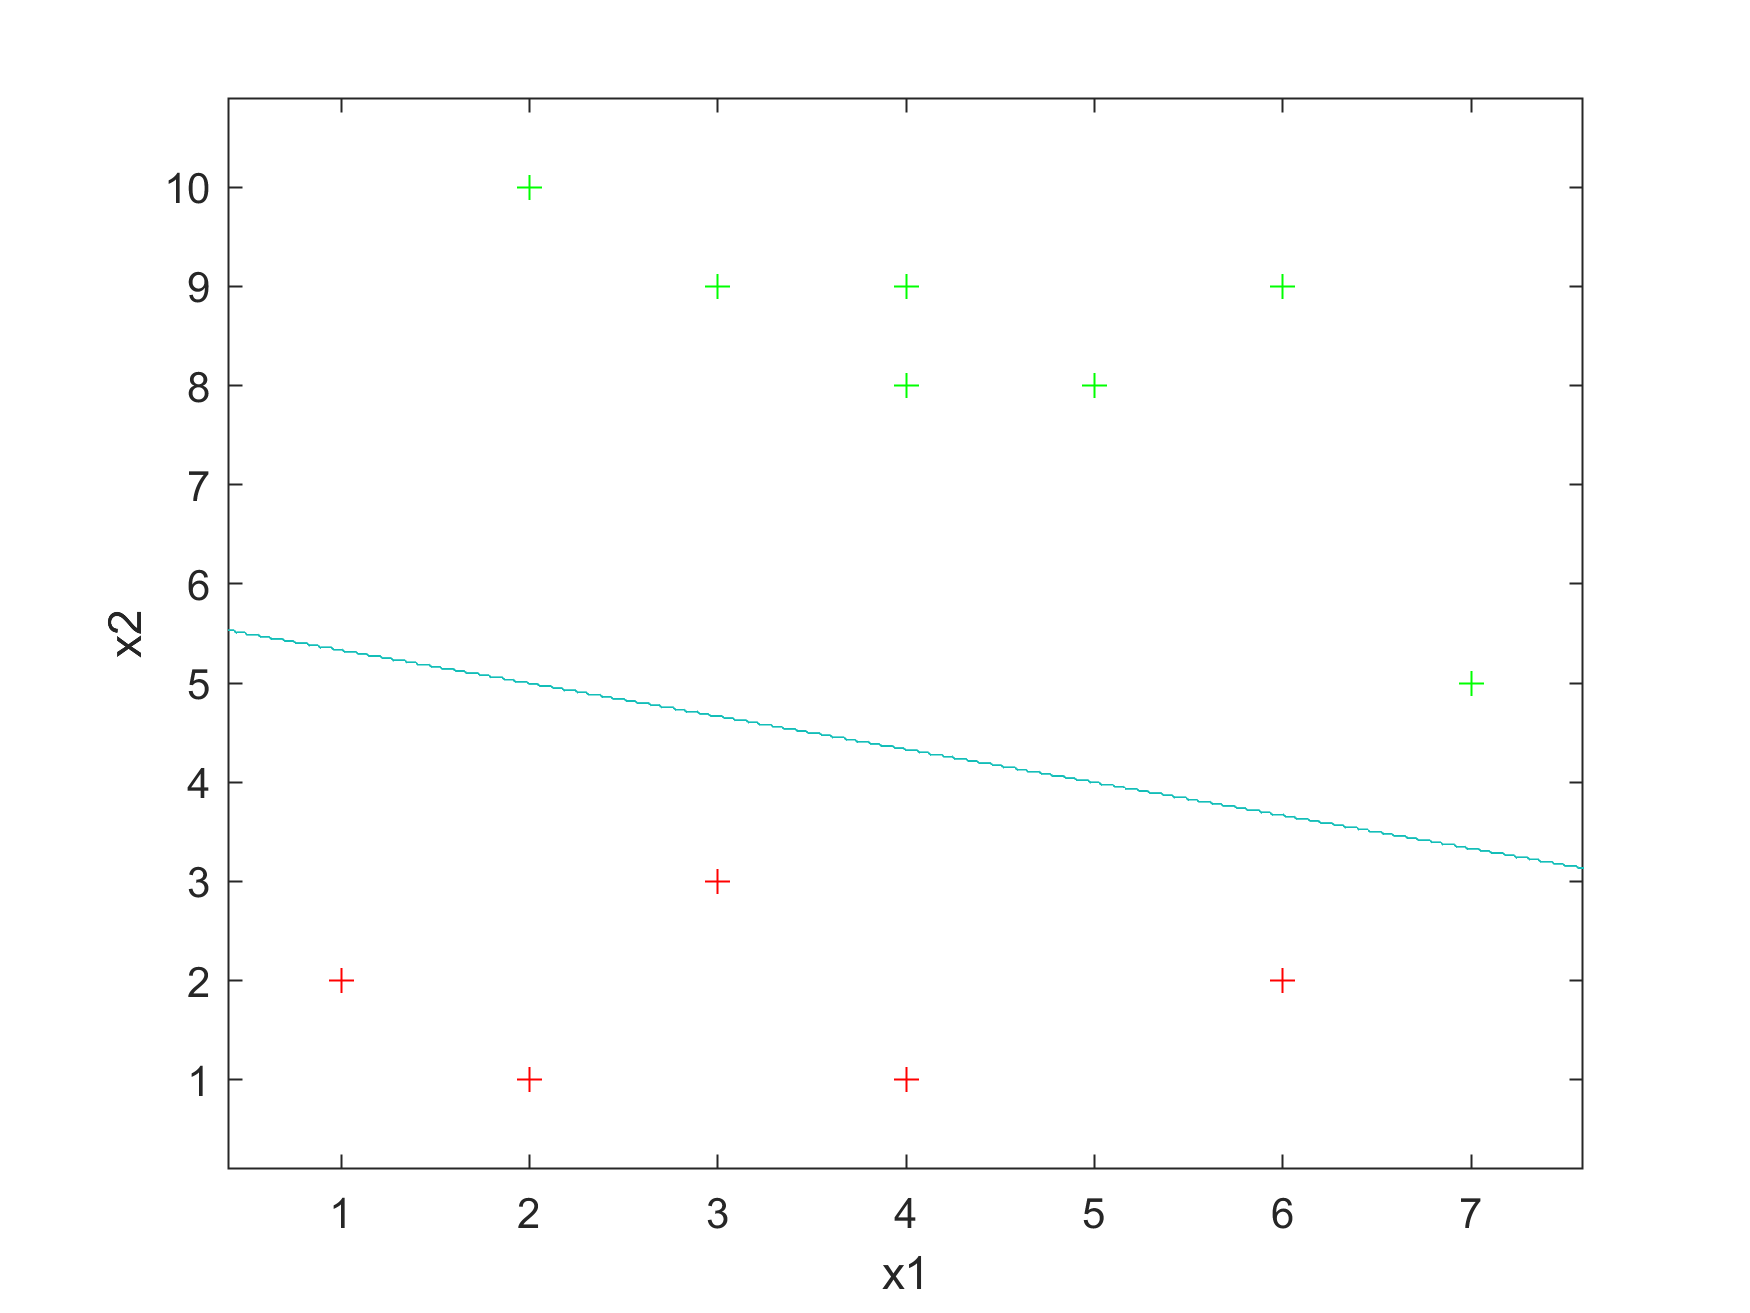
\includegraphics[width = 16cm]{../code/octave/images/svmsimple}
    \caption{Linear separierbarer Datensatz mit Grenze von Hard-Margin SVM}
    \label{fig:hmsvmbsp_simple}
\end{figure}
Wie ersichtlich hat die Grenze, die \glqq hard margin\grqq einen Mindestabstand zu allen Punkten.
\autoref{fig:hmsvm_comp} zeigt den Vergleich zwischen einer Hard-Margin SVM, einem Algorithmus mit Pseudoinversen und $\alpha$-LMS.
\begin{figure}[H]
    \centering
    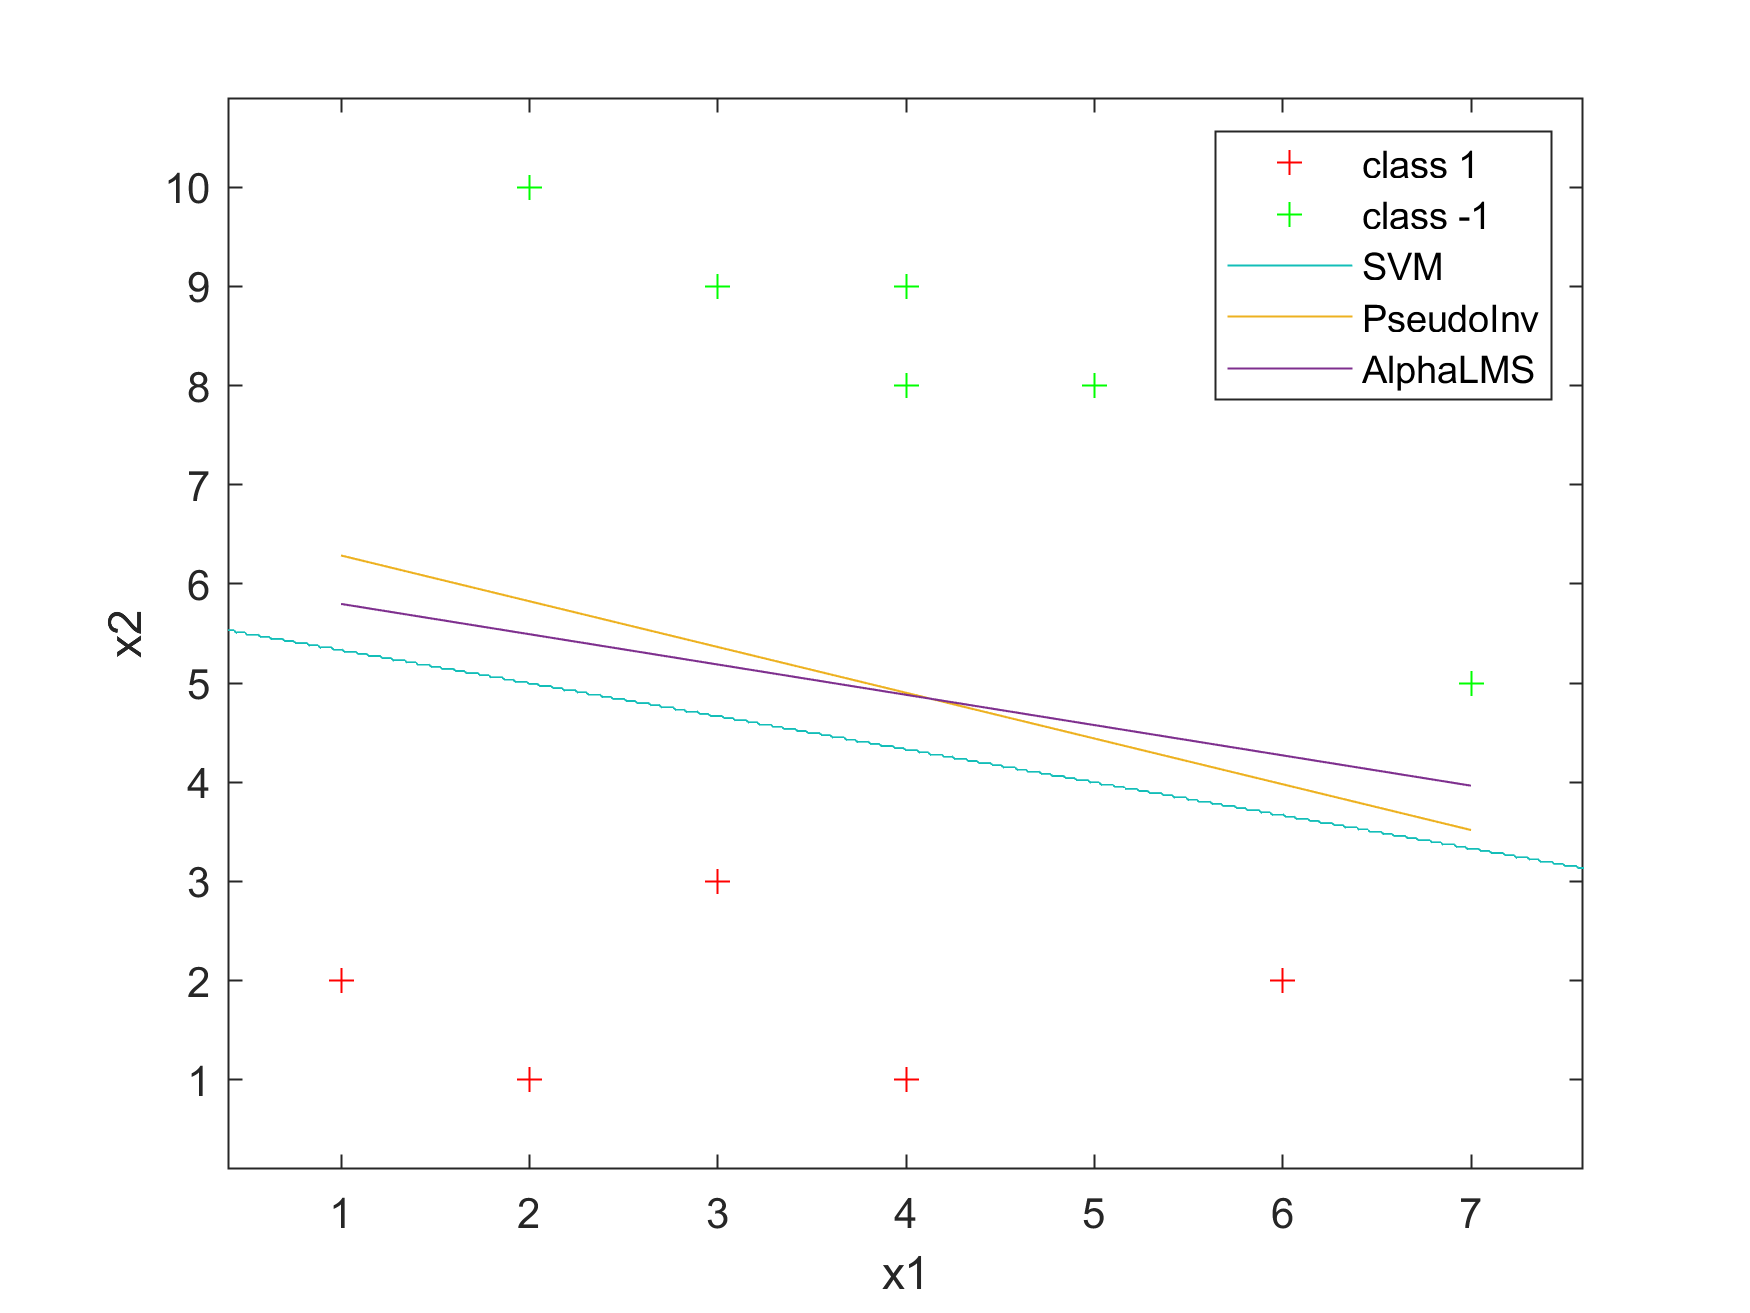
\includegraphics[width = 16cm]{../code/octave/images/linearcompsmall}
    \caption{Linear separierbarer Datensatz mit Grenze von Hard-Margin SVM, Pseudoinverser und $\alpha$-LMS}
    \label{fig:hmsvm_comp}
\end{figure}
Alle Entscheidungsgrenzen trennen den Datensatz sauber.
Im Gegensatz zur Hard-Margin \ac{SVM} ist bei den anderen Algorithmen der Abstand der Punkte zur Grenze unerheblich.

\section{Soft-Margin SVM Pseudocode}\label{sec:smsvmpseudo}
% TODO add after checking hard margin pseudocode (only small differences)

\section{Soft-Margin SVM Beispiel}\label{sec:smscmbsp}
Im Gegensatz zur Hard-Margin \ac{SVM} kann bei der Soft-Margin \ac{SVM} der Mindestabstand, oder genauer der Bestrafungsfaktor für Abweichungen von diesem, eingestellt werden.
So kann mit einer geringen Bestrafung auch bei nichtlinear separierbaren Datensätzen ein gutes Ergebnis erzielt werden, vorausgesetzt die Klassen sind nur leicht durchmischt.
Ein Beispiel, mit einer Grenze von einer Hard-Margin SVM zum Vergleich, ist in \autoref{fig:smsvm_notlinear} dargestellt.
\begin{figure}[H]
    \centering
    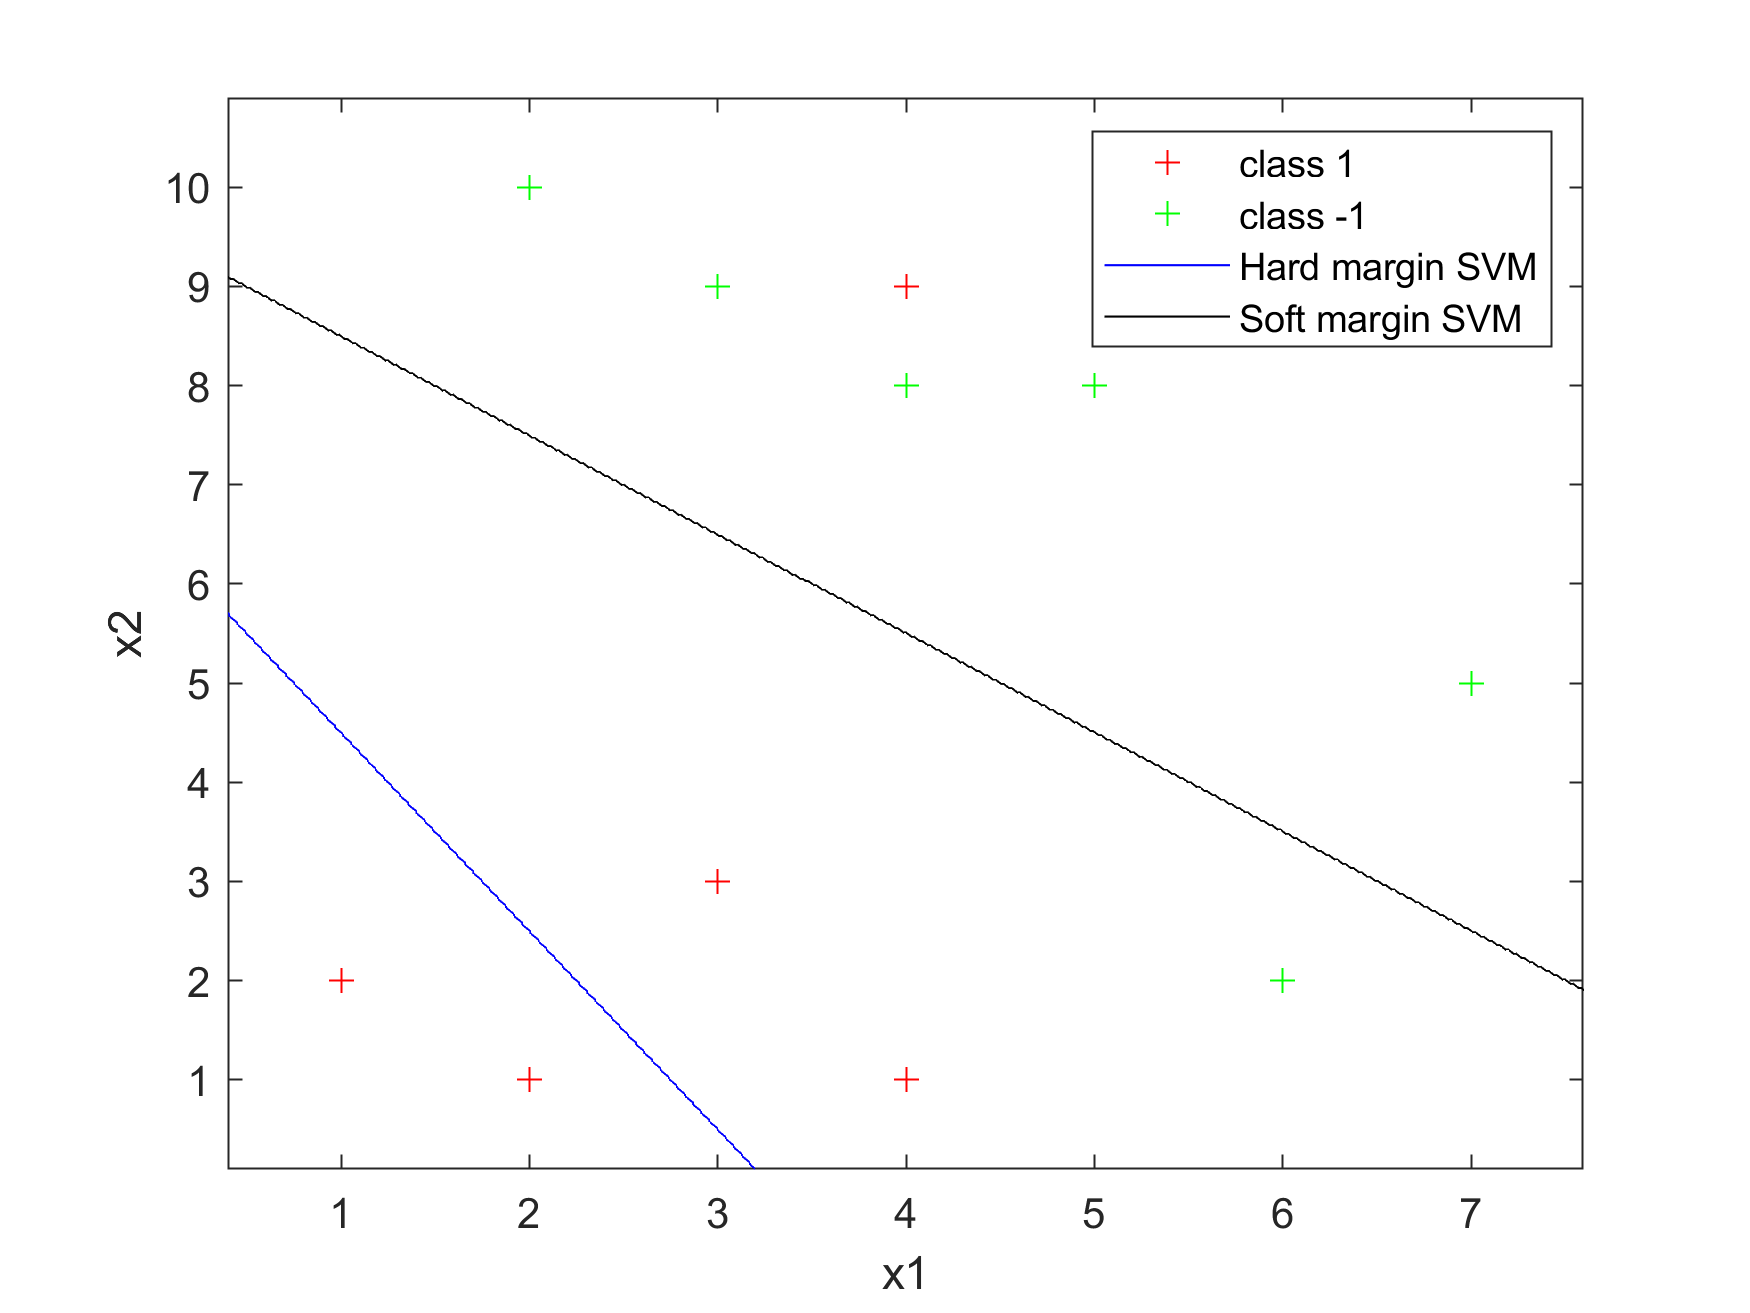
\includegraphics[width = 16cm]{../code/octave/images/svmsimplenotlinear}
    \caption{Nichtlinear separierbarer Datensatz mit Grenze von Hard-Margin \ac{SVM} und Soft-Margin \ac{SVM}}
    \label{fig:smsvm_notlinear}
\end{figure}
Es ist ersichtlich, dass die Soft-Margin \ac{SVM} trotz der zwei Punkte, die eine lineare Trennung verhindern, eine gute Grenze zieht.
Die beiden Ausreißer werden hierbei quasi ignoriert.
Anders bei der Hard-Margin SVM, die durch die Ausreißer stark beeinträchtigt wird und keine Trenngrenze findet.
Wird der Bestrafungsparameter $C$ sehr hoch eingestellt, so verhält sich eine Soft-Margin \ac{SVM} identisch zu einer Hard-Margin \ac{SVM}.

\section{Kernel-Trick, Polynomieller Kernel - Pseudocode}\label{sec:plykernpseudo}
% TODO same as Soft-Margin SVM pseudocode

\section{Kernel-Trick, Polynomieller Kernel - Beispiel}\label{sec:plykernbsp}
Ein polynomieller Kernel der Form $(a x^{T}x' + b)^{Q}$ wird für dieses Beispiel verwendet.
Beim polynomiellen Kernel gilt es herauszufinden, durch welches Polynom sich eine Trennung der eigentlich nichtlinearen Problemstellung erreichen lässt.
Hierfür benötigt man entweder Erfahrung oder Experimente.
Für das folgende Experiment gilt $b = 1, a = 1$, der Exponent $Q$ wird variiert. %TODO mention C=0.1?
\autoref{fig:plykern_qvary} zeigt die Entscheidungsgrenzen für verschiedene $Q$ für den Datensatz KM40M2-NN aus Übung 5b) des Aufgabenblattes. %TODO Referenz?
\begin{figure}[H]
    \centering
    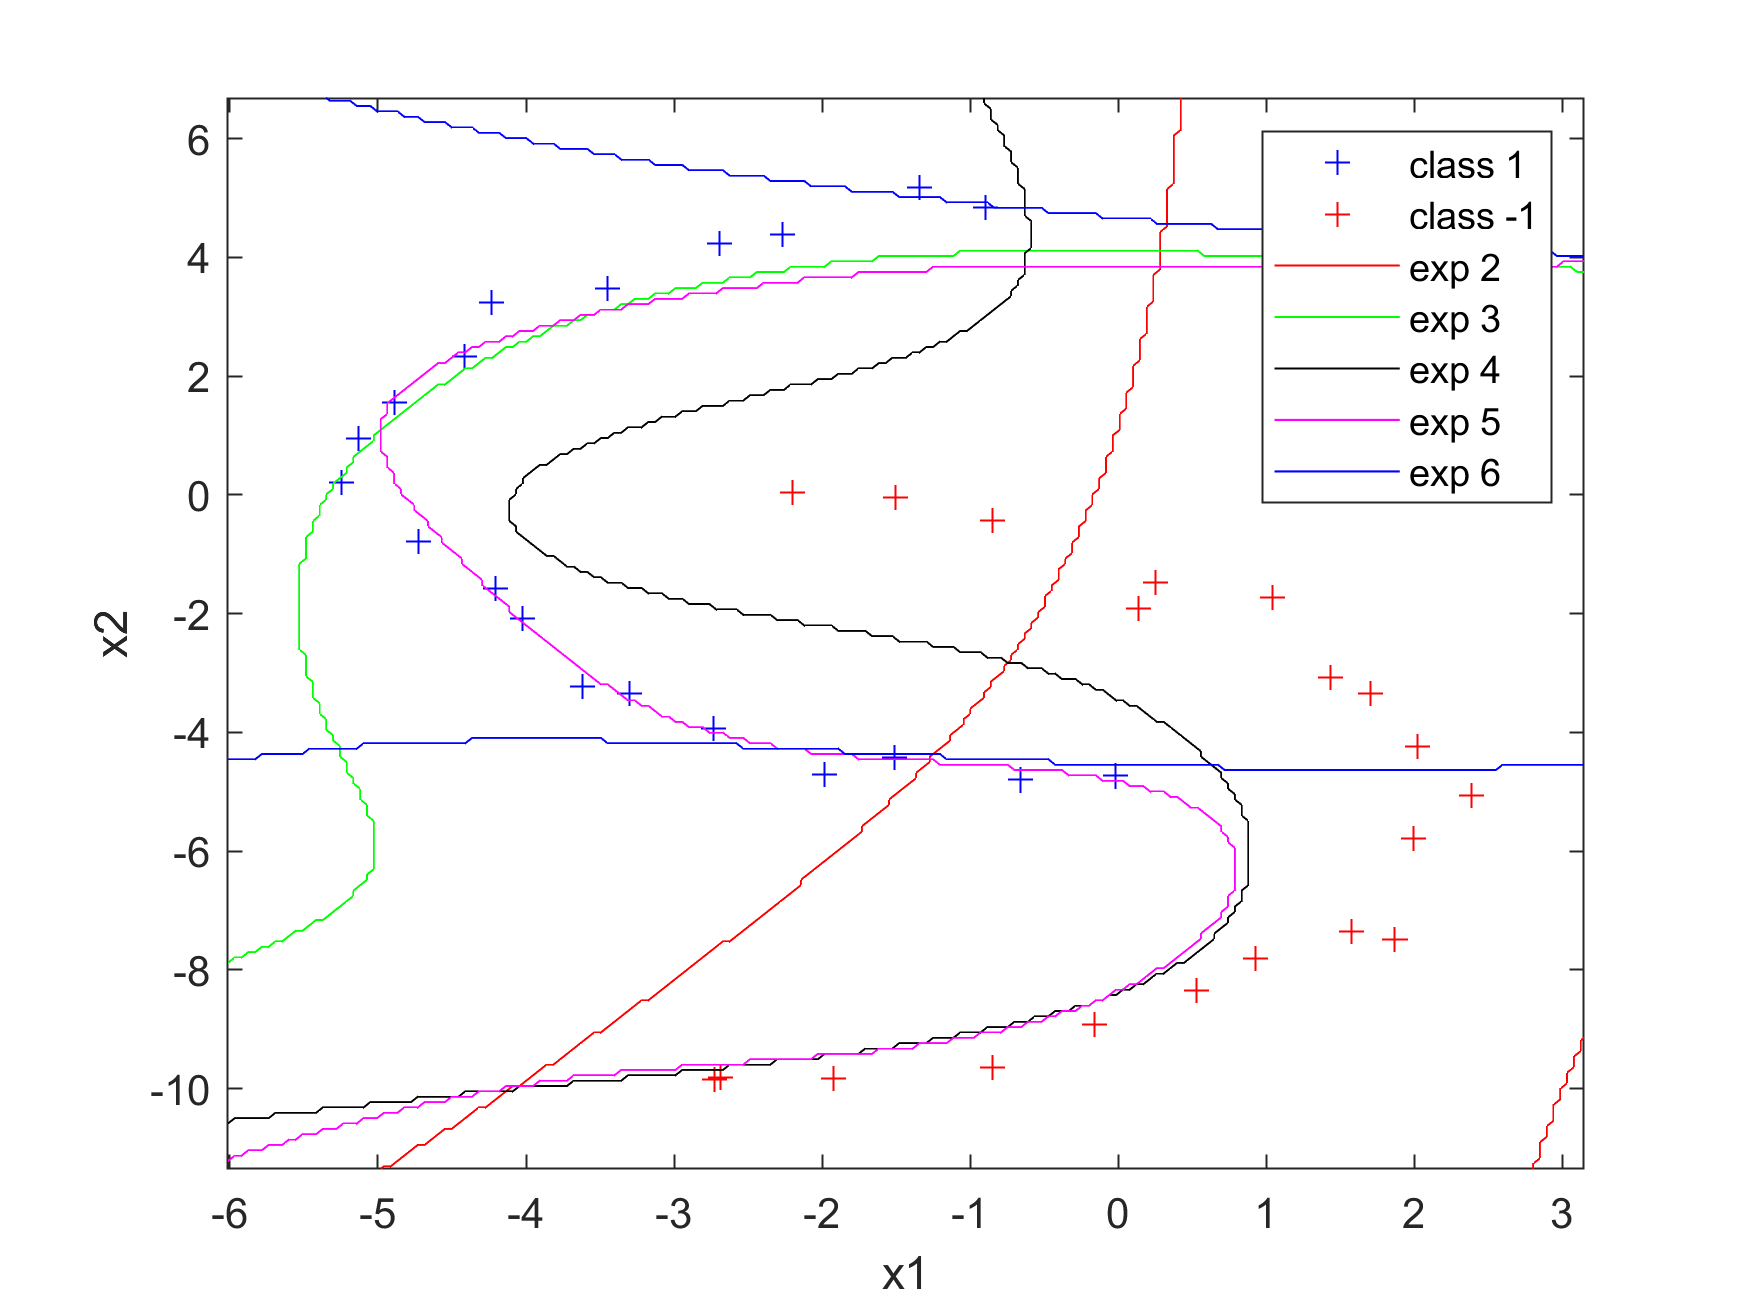
\includegraphics[width = 16cm]{../code/octave/images/kernelexptest}
    \caption{Nichtlinear separierbarer Datensatz mit Grenze von \ac{SVM} mit polynomiellem Kernel für $Q=2,\ldots,6$}
    \label{fig:plykern_qvary}
\end{figure}
Man kann die verschiedenen Grenzen beobachten und graphisch analysieren.
Da sich durch den Kerneltrick der Rechenaufwand in Grenzen hält, kann über die Variation von $Q$ und gegebenenfalls auch $a, b$ gut experimentiert werden, um ein geeignetes Polynom zu finden.
Bei genauerer Betrachtung bietet sich bei diesem Beispiel ein Exponent von $Q=4$ an.
In \autoref{fig:plykern_solve} ist die Entscheidungsgrenze für dieses Polynom abgebildet.
\begin{figure}[H]
    \centering
    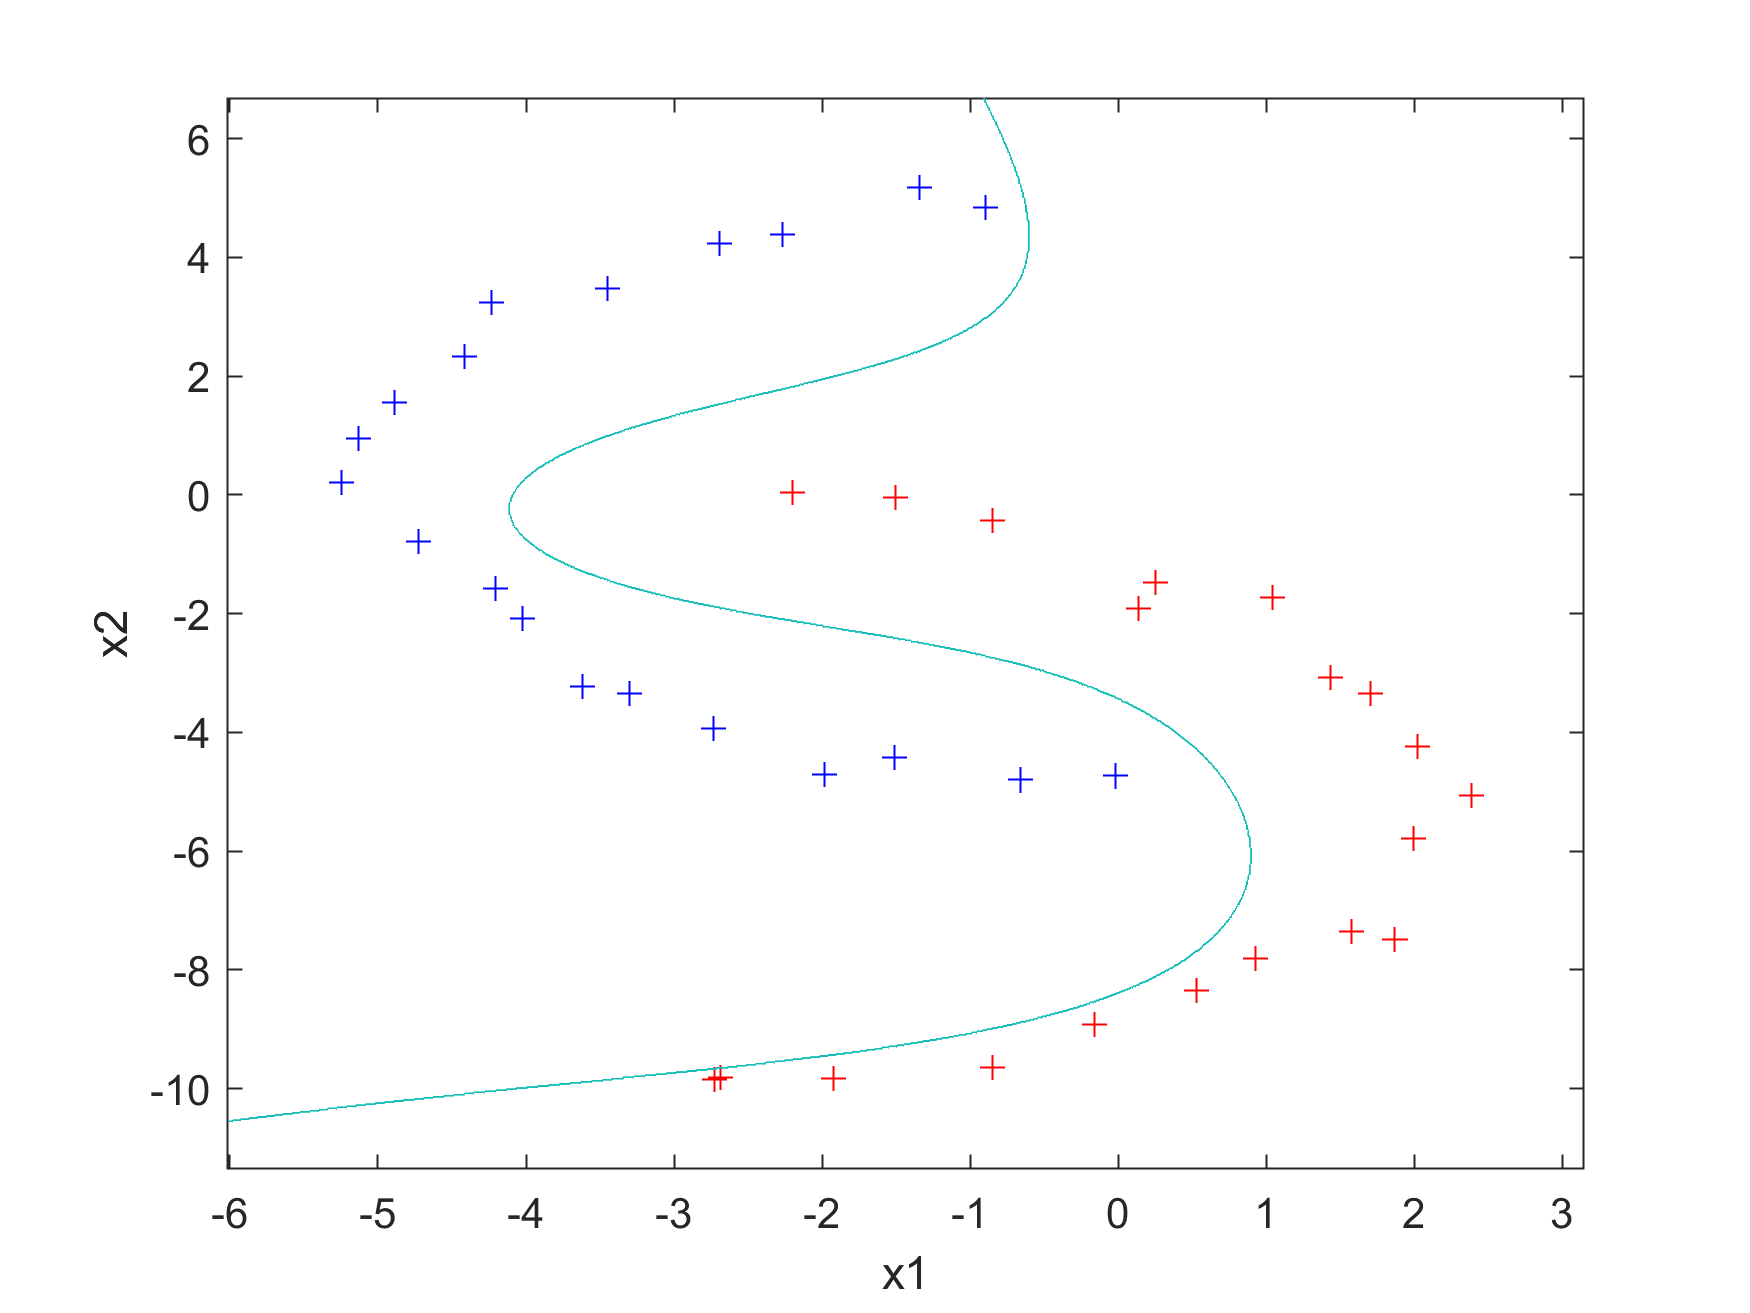
\includegraphics[width = 16cm]{../code/octave/images/sgddatasetkernelsolve}
    \caption{Nichtlinear separierbarer Datensatz mit Grenze von \ac{SVM} mit polynomiellem Kernel für $Q=4$}
    \label{fig:plykern_solve}
\end{figure}
Die Punkte werden, auch bei diesem nichtlinearen Problem, sauber getrennt.

\section{Kernel-Trick, RBF Kernel - Pseudocode}\label{sec:rbfkern_pseudo}
% TODO like poly-kernel

\section{Kernel-Trick, RBF Kernel - Beispiel}\label{sec:rbfkern_bsp}
Anders als beim polynomiellen Kernel muss beim \ac{RBF} Kernel nicht nach einem Polynom gesucht werden.
Dafür muss der Parameter $\gamma$ korrekt eingestellt werden.
% Weiter muss auch auf den Bestrafungsparameter $C$ geachtet werden.
Für $\gamma = 1$ ergibt sich, angewandt auf den Datensatz KM40M2-NN, \autoref{fig:rbfkern_dataset}. %TODO mention C=200?
\begin{figure}[H]
    \centering
    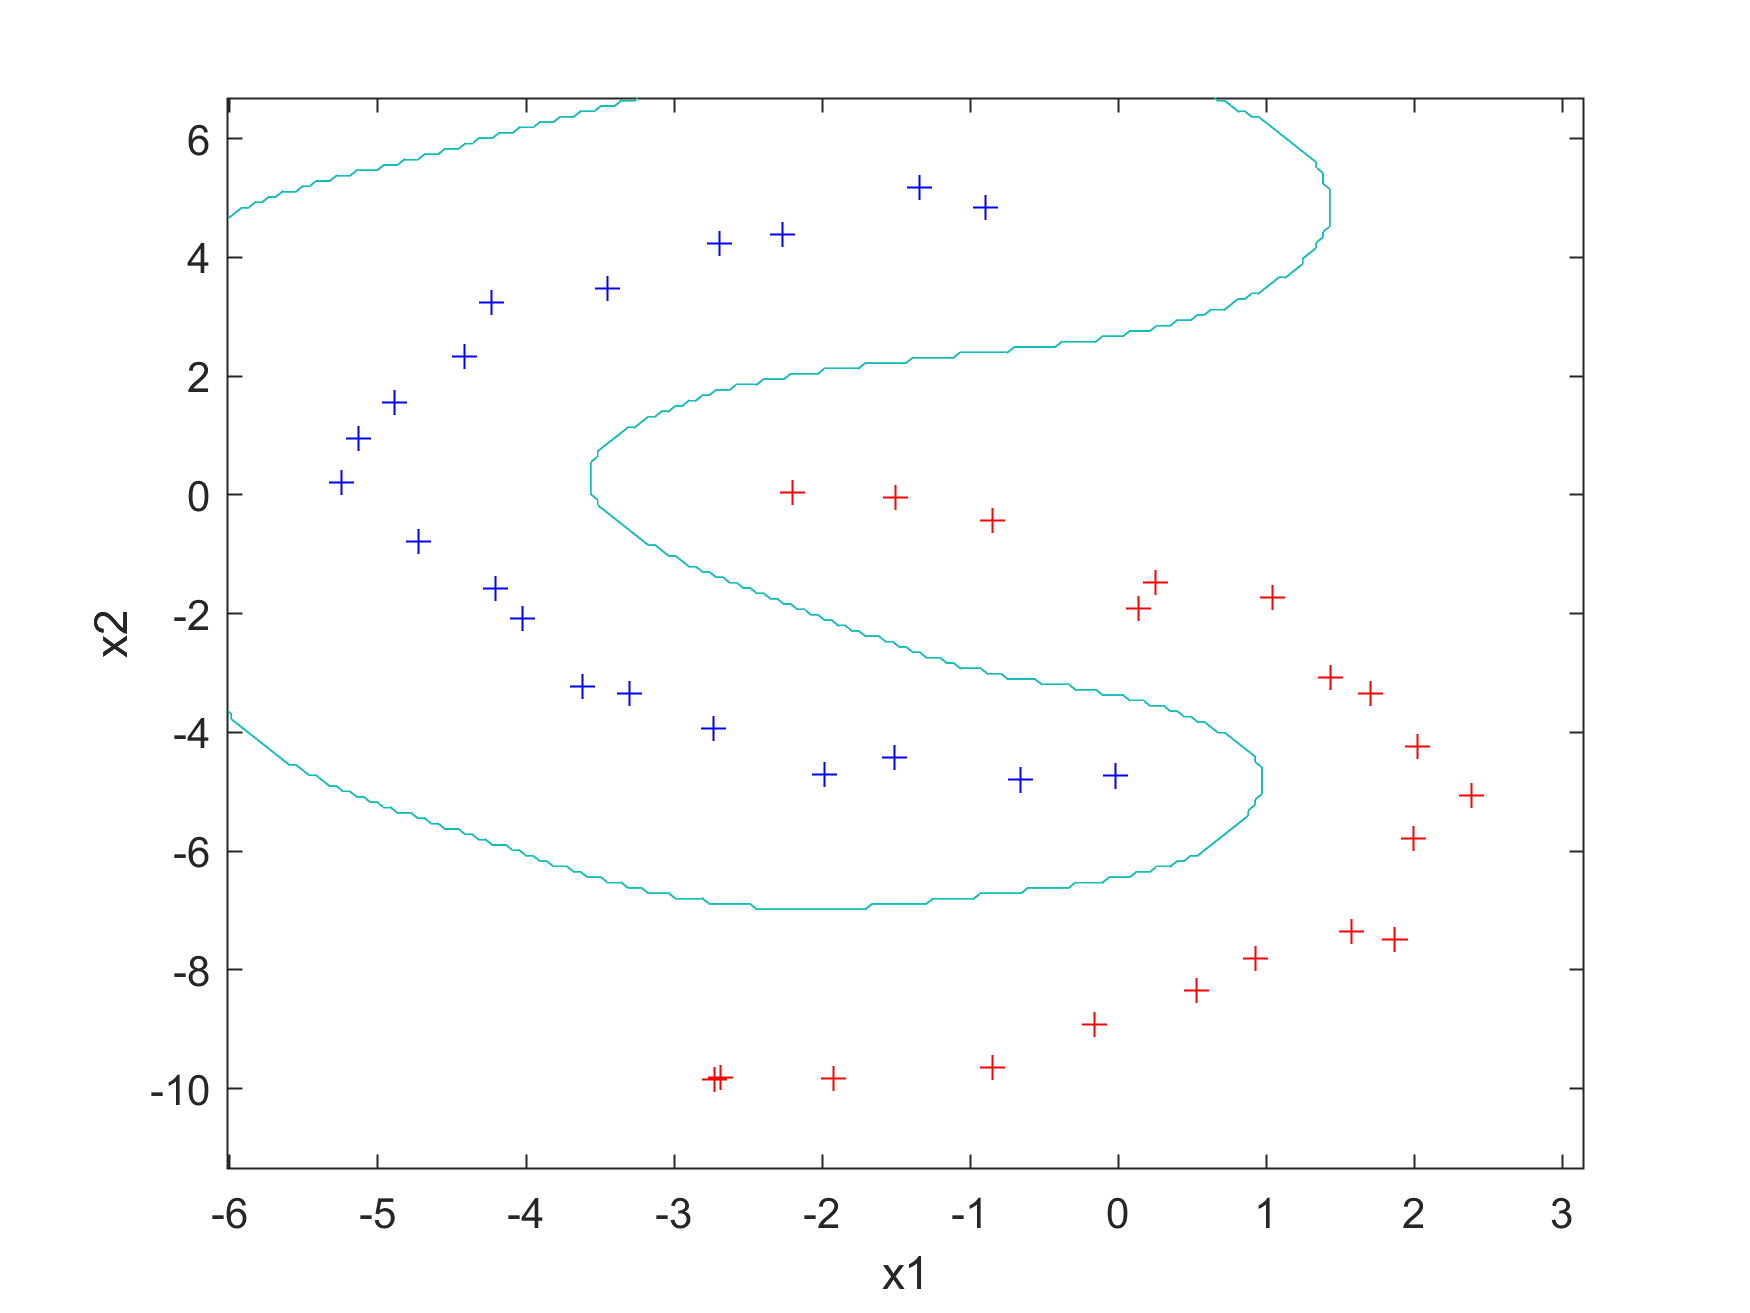
\includegraphics[width = 16cm]{../code/octave/images/sgdrbfkernel}
    \caption{Nichtlinear separierbarer Datensatz mit Grenze von \ac{SVM} mit \ac{RBF}-Kernel für $\gamma=1$}
    \label{fig:rbfkern_dataset}
\end{figure}
Man sieht, dass die Punkte schön getrennt werden.
Auch auffallend ist, dass die Grenze die blauen Punkte quasi umschließt.
Bei einer falschen Einstellung von $\gamma$ könnte es z.B. passieren, dass jeder Punkt eine eigene Grenze bekommt. %TODO zeigen?

% THIS COMMAND ADDS ALL ENTRIES (EVEN UNREFERENCED) TO BIBLIOGRAPHY
\nocite{*}

% Literaturverzeichnis:
\clearpage
\phantomsection
\addcontentsline{toc}{chapter}{Weiterführende Ressourcen}
\printbibliography[title=Weiterführende Ressourcen]

\end{document}
